\documentclass[compress]{beamer}

\usetheme[block=fill]{metropolis}

\usepackage{graphicx} % Allows including images
\usepackage{amsmath,amsfonts,amsthm,amssymb}
\usepackage{color}
\usepackage{xcolor,cancel}
\usepackage{enumitem}
\setitemize{label=\usebeamerfont*{itemize item}%
	\usebeamercolor[fg]{itemize item}
	\usebeamertemplate{itemize item}}
\definecolor{mDarkBrown}{HTML}{604c38}
\definecolor{mDarkTeal}{HTML}{23373b}
\definecolor{mLightBrown}{HTML}{EB811B}
\definecolor{mMediumBrown}{HTML}{C87A2F}
\definecolor{mygreen}{HTML}{98C2B9}
\definecolor{myyellow}{HTML}{DFD79C}
\definecolor{myblue}{HTML}{8CA7CC}
\definecolor{kern}{HTML}{8CC2B7}


\usepackage{float}
\usepackage{framed}
\usepackage{epsfig}
\usepackage{graphicx}
\usepackage{subcaption}
\usepackage{ulem}
\usepackage{hhline}
\usepackage{multirow}
\usepackage{comment}   
\usepackage{bbm}
\usepackage{tikz}   
\def\Put(#1,#2)#3{\leavevmode\makebox(0,0){\put(#1,#2){#3}}}
\newcommand*\mystrut[1]{\vrule width0pt height0pt depth#1\relax}
\newcommand{\eqdef}{\mathbin{\stackrel{\rm def}{=}}}


\newcommand{\bs}[1]{\boldsymbol{#1}}
\newcommand{\bv}[1]{\mathbf{#1}}
\newcommand{\R}{\mathbb{R}}
\newcommand{\E}{\mathbb{E}}

\DeclareMathOperator*{\argmin}{arg\,min}
\DeclareMathOperator*{\argmax}{arg\,max}
\DeclareMathOperator{\nnz}{nnz}
\DeclareMathOperator{\diag}{diag}
\DeclareMathOperator{\Var}{Var}
\DeclareMathOperator{\sinc}{sinc}
\DeclareMathOperator{\sign}{sign}
\DeclareMathOperator{\dist}{dist}
\DeclareMathOperator{\mv}{mv}
\DeclareMathOperator{\sgn}{sgn}
\DeclareMathOperator{\step}{step}
\DeclareMathOperator{\gap}{gap}
\DeclareMathOperator{\poly}{poly}
\DeclareMathOperator{\tr}{tr}
\DeclareMathOperator{\orth}{orth}
\newcommand{\norm}[1]{\|#1\|}
\captionsetup[subfigure]{labelformat=empty}
\captionsetup[figure]{labelformat=empty}
\DeclareMathOperator*{\lmin}{\lambda_{min}}
\DeclareMathOperator*{\lmax}{\lambda_{max}}

\newcommand{\specialcell}[2][c]{%
  \begin{tabular}[#1]{@{}c@{}}#2\end{tabular}}
\newcommand{\specialcellleft}[2][c]{%
\begin{tabular}[#1]{@{}l@{}}#2\end{tabular}
}

\newtheorem{claim}[theorem]{Claim}

\usepackage{tabstackengine}
\stackMath


%----------------------------------------------------------------------------------------
%	TITLE PAGE
%----------------------------------------------------------------------------------------

\title{CS-GY 6763: Lecture 7 \\ Second Order Conditions, Online and Stochastic Gradient Decent}
\author{NYU Tandon School of Engineering, Prof. Christopher Musco}
\date{}

\begin{document}

\begin{frame}
	\titlepage 
\end{frame}

\metroset{titleformat=smallcaps}

\begin{frame}[t]
	\frametitle{administrative}
		Midterm in class next Wednesday. 
		\begin{itemize}
			\item List of topics covered and practice problems will be posted on the course webpage. 
			\item You are allowed a double sided sheet of paper. 
			\item If you are taking it at the Moses Center, please send me an email just to make sure I don't forget.
			\item I will go over Problem Set 2 in office hours on Monday and record it. Recording of Majid going over Problem Set 1 already posted. 
		\end{itemize}
\end{frame}

\begin{frame}[t]
	\frametitle{gradient descent recap}
	\textbf{First Order Optimization:} Given a function $f$ and a constraint set $\mathcal{S}$, assume we have:
	\begin{itemize}
		\item \textbf{Function oracle}: Evaluate $f(\bv{x})$ for any $\bv{x}$. 
		\item \textbf{Gradient oracle}: Evaluate $\nabla f(\bv{x})$ for any $\bv{x}$.
		\item \textbf{{Projection oracle}}: Evaluate $P_{\mathcal{S}}(\bv{x})$ for any $\bv{x}$.
	\end{itemize}
\begin{center}
	\textbf{Goal:} Find $\hat{\bv{x}}\in \mathcal{S}$ such that $f(\hat{\bv{x}}) \leq \min_{\bv{x}\in \mathcal{S}}f(\bv{x})+\epsilon$.
\end{center}
\end{frame}

\begin{frame}[t]
	\frametitle{gradient descent recap}
	\textbf{Projected gradient descent:}
	\begin{itemize}
		\item Select starting point $\bv{x}^{(0)}$, learning rate $\eta$. 
		\item For $i = 0,\ldots, T$:
		\begin{itemize}
			\item $\bv{z} = \bv{x}^{(i)} - \eta \nabla f(\bv{x}^{(i)})$
			\item $\bv{x}^{(i+1)} = P_\mathcal{S}(\bv{z})$
		\end{itemize}
		\item Return $\hat{\bv{x}} = \argmin_{i} f(\bv{x}^{(i)})$.
	\end{itemize}
\end{frame}

\begin{frame}[t]
	\frametitle{gradient descent recap}
	\textbf{Conditions for convergence:}
	\begin{itemize}
		\item \textbf{Convexity:} $f$ is a convex function, $\mathcal{S}$ is a convex set. 
		\item \textbf{Bounded initial distance:} 
		\begin{align*}
			\|\bv{x}^{(0)} - \bv{x}^*\|_2 \leq \alert{R}
		\end{align*}
		\item \textbf{Bounded gradients (Lipschitz function)}: 
		\begin{align*}
			\|\nabla f(\bv{x})\|_2 \leq \alert{G} \text{ for all } \bv{x}\in \mathcal{S}.
		\end{align*}
	\end{itemize}

\textbf{Theorem:} Projected Gradient Descent returns $\hat{\bv{x}}$ with $f(\hat{\bv{x}}) \leq \min_{\bv{x}\in \mathcal{S}}f(\bv{x})+\epsilon$ after
\begin{align*}
	T = \frac{R^2G^2}{\epsilon^2}
\end{align*}
iterations. 
\end{frame}

\begin{frame}[t]
	\frametitle{other convergence guarantees}
	Convexity: 
	\begin{align*}
		0 \leq \left[f(\bv{y}) - f(\bv{x})\right] - \nabla f(\bv{x})^T(\bv{y} - \bv{x})
	\end{align*}
$\beta$-smoothness:
	\begin{align*}
		\left[f(\bv{y}) - f(\bv{x})\right] - \nabla f(\bv{x})^T(\bv{y} - \bv{x}) \leq \alert{\frac{\beta}{2}}\|\bv{x} - \bv{y}\|_2^2.
	\end{align*}
	\textbf{Number of iterations for $\epsilon$ error:}
\begin{center}
	\begin{tabular}{c|cc}
		& $G$-Lipschitz & $\beta$-smooth   \\ \hline
		$R$ bounded start & $O\left(\frac{G^2R^2}{\epsilon^2}\right)$ & $O\left(\frac{\beta R^2}{\epsilon}\right)$ \\
		$\alpha$-strong convex  & $O\left(\frac{G^2}{\alpha\epsilon}\right)$ & $O\left(\frac{\beta}{\alpha}\log(R/\epsilon)\right)$
	\end{tabular}
\end{center}
\end{frame}

\begin{frame}[t]
	\frametitle{strong convexity}
	\begin{definition}[$\alpha$-strongly convex]
		A convex function $f$ is $\alert{\alpha}$-strongly convex if, for all $\bv{x}$, $\bv{y}$
		\begin{align*}
			\frac{\alpha}{2}\|\bv{x} - \bv{y}\|_2^2  \leq \left[f(\bv{y}) - f(\bv{x})\right] - \nabla f(\bv{x})^T(\bv{y} - \bv{x})
		\end{align*}
	\end{definition}
	For a twice-differentiable scalar function $f$, equivalent to $f''(x) \geq \alpha$.  
	\vspace{-2em}
	\begin{center}
	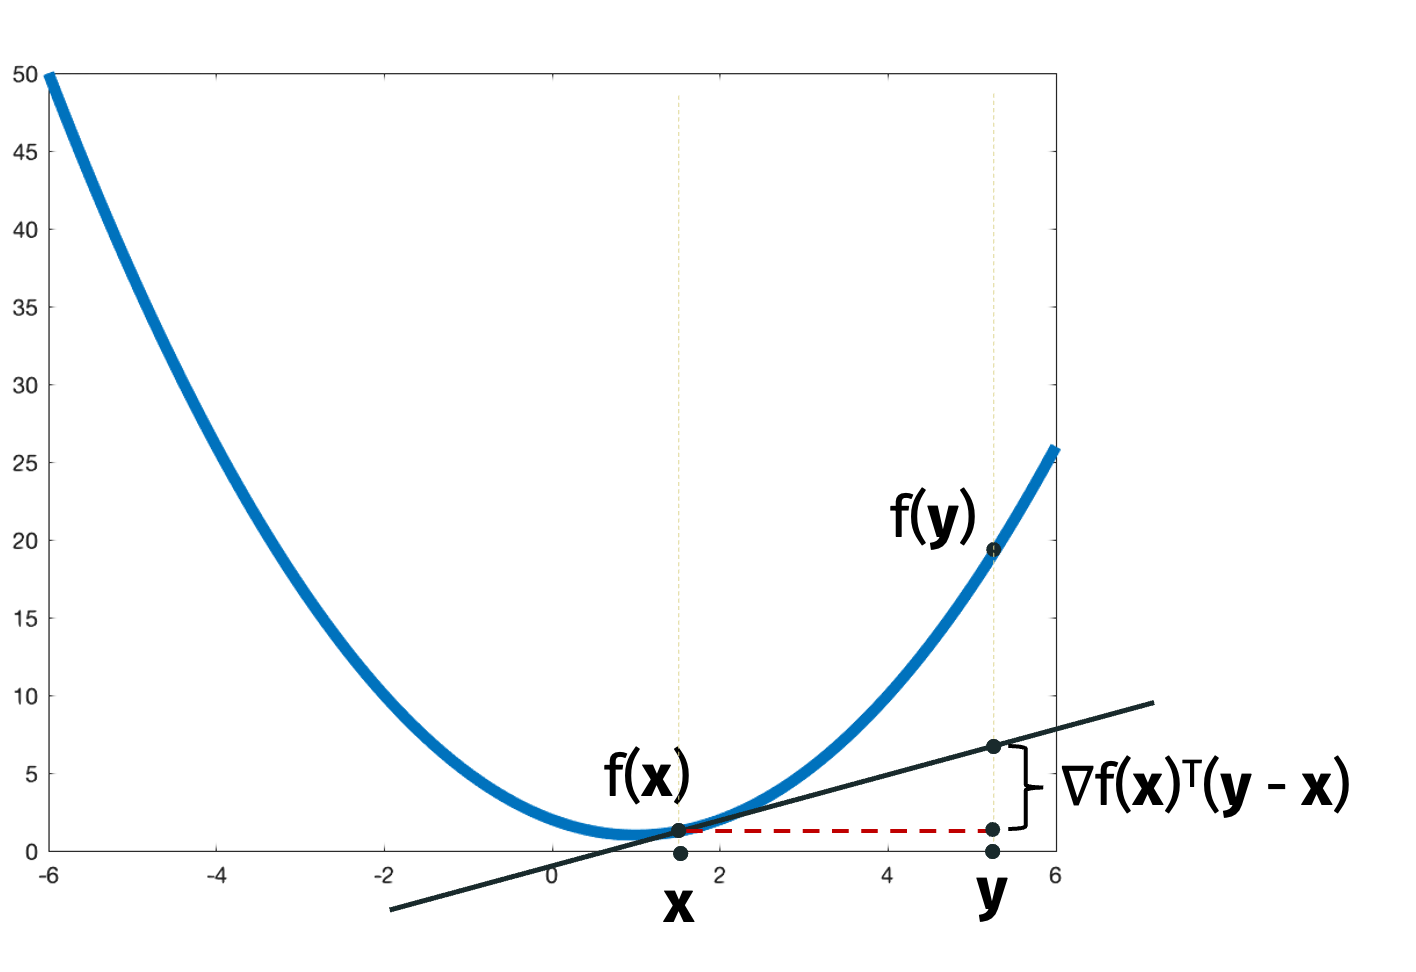
\includegraphics[width=.6\textwidth]{smoothness_image.png}
\end{center}	

\end{frame}



\begin{frame}[t]
	\frametitle{gd for strongly convex function}
	\textbf{Gradient descent for strongly convex functions:}
	\begin{itemize}
		\item Choose number of steps $T$.
		\item For $i = 1,\ldots, T$:
		\begin{itemize}
			\item $\eta = \frac{2}{\alpha\cdot(i+1)}$
			\item $\bv{x}^{(i+1)} = \bv{x}^{(i)} - \eta \nabla f(\bv{x}^{(i)})$
		\end{itemize}
		\item Return $\hat{\bv{x}} = \argmin_{\bv{x}^{(i)}} f(\bv{x}^{(i)})$. 
		%		\item Alternatively, return $\hat{\bv{x}} = \sum_{i=1}^T \frac{2i}{T(T+1)} \bv{x}^{(i)}$.
	\end{itemize}
\end{frame}

\begin{frame}[t]
	\frametitle{convergence guarantee}
	\begin{theorem}[GD convergence for $\alpha$-strongly convex functions.]
		Let $f$ be an \alert{$\alpha$}-strongly convex function and assume we have that, for all $\bv{x}$, $\|\nabla f(\bv{x})\|_2 \leq \alert{G}$. If we run GD for $T$ steps (with adaptive step sizes) we have:
		\begin{align*}
			f(\hat{\bv{x}}) - f(\bv{x}^*) \leq \frac{2G^2}{\alpha(T-1)} 
		\end{align*} 
	\end{theorem}
	\textbf{Corollary}: If \alert{$T = O\left(\frac{G^2}{\alpha \epsilon}\right)$} we have $f(\hat{\bv{x}}) - f(\bv{x}^*) \leq \epsilon$
\end{frame}

\begin{frame}[t]
	\frametitle{convergence guarantee}
	\begin{center}
		We could also have that $f$ is both $\beta$-smooth and $\alpha$-strongly convex.
	\end{center}
	\begin{align*}
		\alert{\frac{\alpha}{2}}\|\bv{x} - \bv{y}\|_2^2 \leq \left[f(\bv{y}) - f(\bv{x})\right] - \nabla f(\bv{x})^T(\bv{y} - \bv{x}) \leq \alert{\frac{\beta}{2}}\|\bv{x} - \bv{y}\|_2^2.
	\end{align*}
	\vspace{-2em}
	\begin{center}
		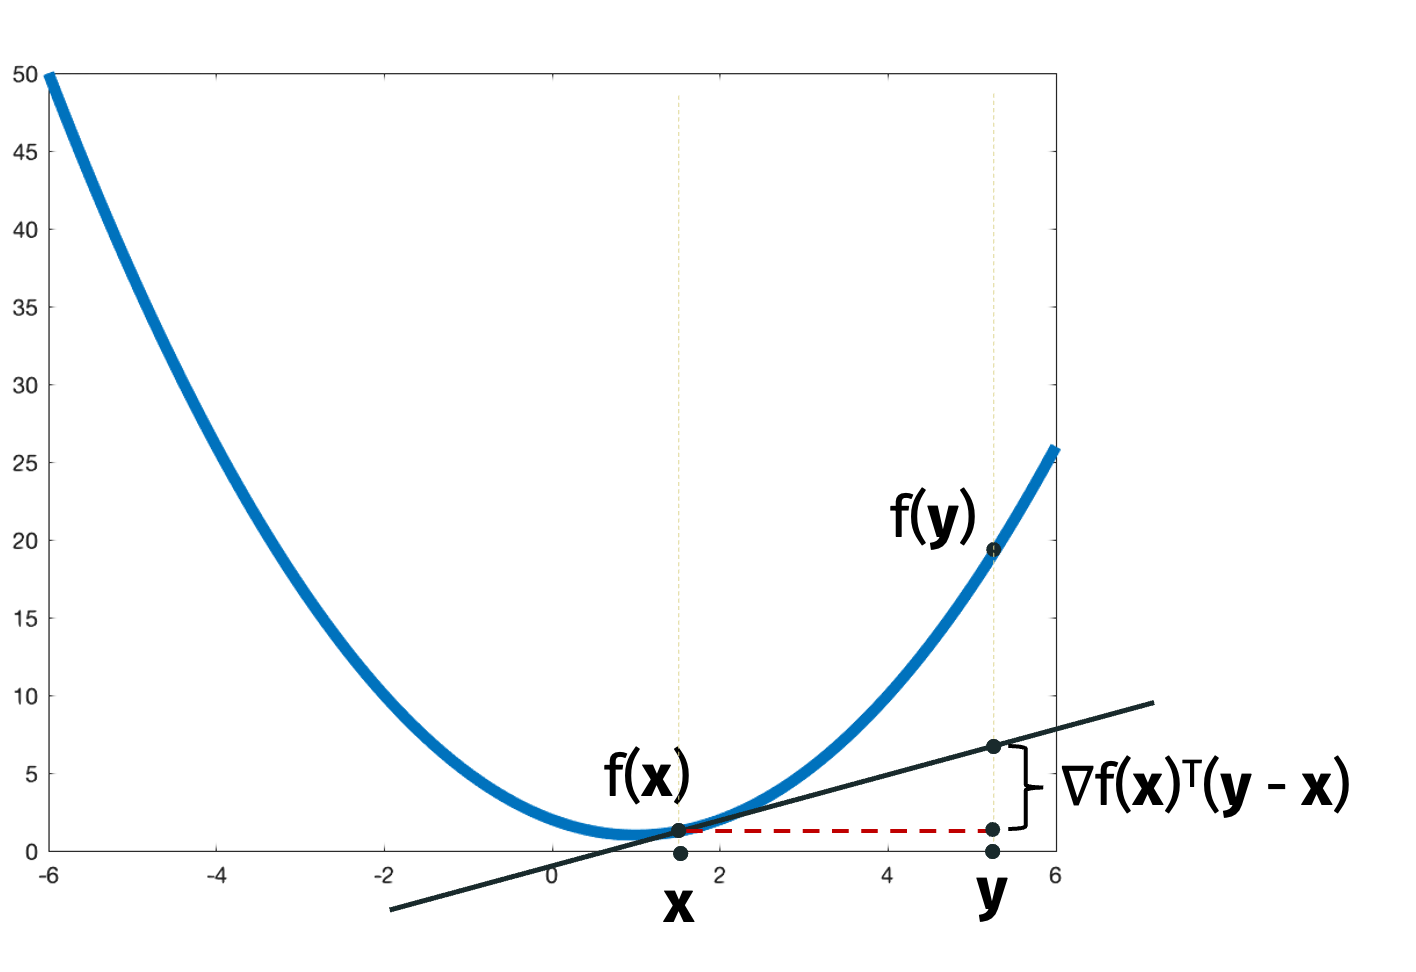
\includegraphics[width=.6\textwidth]{smoothness_image.png}
	\end{center}	
	
\end{frame}

\begin{frame}[t]
	\frametitle{convergence guarantee}
	\begin{align*}
		\alert{\frac{\alpha}{2}}\|\bv{x} - \bv{y}\|_2^2 \leq\left[f(\bv{y}) - f(\bv{x})\right] - \nabla f(\bv{x})^T(\bv{y} - \bv{x}) \leq \alert{\frac{\beta}{2}}\|\bv{x} - \bv{y}\|_2^2.
	\end{align*}
	
	\begin{theorem}[GD for $\beta$-smooth, $\alpha$-strongly convex.]
		Let $f$ be a $\beta$-smooth and $\alpha$-strongly convex function. If we run GD for $T$ steps (with step size $\eta = \frac{1}{\beta}$) we have:
		\begin{align*}
			\|\bv{x}^{(T)} - \bv{x}^*\|_2^2 \leq e^{-T \frac{\alpha}{\beta}} \|\bv{x}^{(0)} - \bv{x}^*\|_2^2
		\end{align*} 
	\end{theorem}	
	\begin{center}
		\alert{$\kappa = \frac{\beta}{\alpha}$} is called the ``condition number'' of $f$. 
		
		\textbf{Is it better if $\kappa$ is large or small?}
	\end{center}
\end{frame}

\begin{frame}[t]
	\frametitle{smooth and strongly convex}
	\textbf{Converting to more familiar form:}
	Using that fact the $\nabla f(\bv{x}^*) = \bv{0}$ along with
	\begin{align*}
		{\frac{\alpha}{2}}\|\bv{x} - \bv{y}\|_2^2 \leq  \left[f(\bv{y}) - f(\bv{x})\right] - \nabla f(\bv{x})^T(\bv{y} - \bv{x}) \leq {\frac{\beta}{2}}\|\bv{x} - \bv{y}\|_2^2, 
	\end{align*}
	we have:
	\begin{align*}
		\|\bv{x}^{(T)} - \bv{x}^*\|_2^2 &\geq \frac{2}{\beta} \left[f(\bv{x}^{(T)}) - f(\bv{x}^*)\right].
	\end{align*}	
We also assume
\begin{align*}
			\|\bv{x}^{(0)} - \bv{x}^*\|_2^2 &\leq R.
\end{align*}
\end{frame}

\begin{frame}[t]
	\frametitle{convergence guarantee}
	\begin{theorem}[GD for $\beta$-smooth, $\alpha$-strongly convex.]
		Let $f$ be a $\beta$-smooth and $\alpha$-strongly convex function. If we run GD for $T$ steps (with step size $\eta = \frac{1}{\beta}$) we have:
		\begin{align*}
			f(\bv{x}^{(T)}) - f(\bv{x}^*)  \leq \frac{\beta}{\alpha} e^{-T\frac{\alpha}{\beta}} \cdot  \left[f(\bv{x}^{(0)}) - f(\bv{x}^*)\right]
		\end{align*} 
	\end{theorem}	
%	
%	\textbf{Corollary}: 
%	If \alert{$T = O\left(\frac{\beta}{\alpha}\log(\beta/\alpha \epsilon)\right) =  O(\kappa\log(\kappa/\epsilon))$ } we have:
%	\begin{align*}
%		f({\bv{x}}^{(T)}) - f(\bv{x}^*) \leq \epsilon \left[f(\bv{x}^{(0)}) - f(\bv{x}^*)\right]
%	\end{align*}
	
	\textbf{Corollary}: 
	If \alert{$T = O\left(\frac{\beta}{\alpha}\log(R\beta/\epsilon)\right)$} we have:
	\begin{align*}
		f({\bv{x}}^{(T)}) - f(\bv{x}^*) \leq \epsilon
	\end{align*}
	Only depend on $\log(1/\epsilon)$ instead of on $1/\epsilon$ or $1/\epsilon^2$!
\end{frame}

\begin{frame}[t]
	\frametitle{all convergence guarantees}
We're going to prove this theorem for the special case of a quadratic function:
\begin{align*}
	\|\bv{A}\bv{x}- \bv{b}\|_2^2.
\end{align*}

Underwhelming, yes, but the analysis is really helpful pedagogically! Also if there is one class of algorithms that use more of the worlds computing power than training neural networks, it's GD like iterative methods for solving linear systems.
\end{frame}

\begin{frame}[t]
	\frametitle{the hessian}
	Let $f$ be a twice differentiable function from $\R^d \rightarrow \R$. Let the \textbf{\alert{Hessian}} $\bv{H} = \nabla^2 f(\bv{x})$ contain all of its second derivatives at a point $\bv{x}$. So $\bv{H}\in \R^{d\times d}$.  We have:
	\begin{align*}
		\bv{H}_{j,k} = \left[\nabla^2 f(\bv{x})\right]_{j,k} = \frac{\partial^2 f}{\partial x_j x_k}. 
	\end{align*}
	
	For vector $\bv{x}, \bv{v}$:
	\begin{align*}
		\nabla f(\bv{x} + t\bv{v}) \approx \nabla f(\bv{x}) + t\left[\nabla^2 f(\bv{x})\right]\bv{v}.
	\end{align*}
\end{frame}

\begin{frame}[t]
	\frametitle{the hessian}
	Let $f$ be a twice differentiable function from $\R^d \rightarrow \R$. Let the \textbf{\alert{Hessian}} $\bv{H} = \nabla^2 f(\bv{x})$ contain all of its second derivatives at a point $\bv{x}$. So $\bv{H}\in \R^{d\times d}$.  We have:
	\begin{align*}
		\bv{H}_{j,k} = \left[\nabla^2 f(\bv{x})\right]_{j,k} = \frac{\partial^2 f}{\partial x_j x_k}. 
	\end{align*}
	
	\textbf{Example:} $f(\bv{x}) = \sum_{i=1}^n \left(\bv{x}^T\bv{a}^{(i)} - {y}^{(i)}\right)^2 = \|\bv{A}\bv{x} - \bv{y}\|_2^2$
	\begin{align*}
		\frac{\partial f}{\partial x_j} &= \sum_{i=1}^n 2\left(\bv{x}^T\bv{a}^{(i)} - {y}^{(i)}\right)\cdot a^{(i)}_j \\
		\frac{\partial^2 f}{\partial x_k\partial x_j} &= \sum_{i=1}^n 2a^{(i)}_k  a^{(i)}_j \\
		\bv{H} &=  
	\end{align*}
\end{frame}



\begin{frame}[t]
	\frametitle{alternative derivation}
	$f(\bv{x}) = \|\bv{A}\bv{x} - \bv{b}\|_2^2$. Recall that $\nabla f(\bv{x}) = 2\bv{A}^T(\bv{A}\bv{x}-\bv{b}).$
	
\end{frame}

\begin{frame}[t]
	\frametitle{convexity in 1-d}
	A twice-differentiable function $f:\R\rightarrow R$ is :
	\begin{itemize}
		\item convex if and only if $f''(x)\geq 0$ for all $x$.
		\item $\beta$-smooth if $f''(x) \leq \beta$. 
		\item $\alpha$-strongly convex if $f''(x) \geq \alpha$. 
	\end{itemize}
	\vspace{8em}
	How do these statements generalize to the case when $f$ has a vector in put, so the second derivative is a matrix $\bv{H}$?
\end{frame}

\begin{frame}[t]
	\frametitle{hessian matrices and positive semidefiniteness}
	\textbf{Claim:} If $f$ is twice differentiable, then it is convex if and only if the matrix $\bv{H} = \nabla^2 f(\bv{x})$ is \emph{positive semidefinite} for all $\bv{x}$. 
	
	\begin{definition}[Positive Semidefinite (PSD)]
		A square, symmetric matrix $\bv{H}\in \R^{d\times d}$ is \emph{positive semidefinite} (PSD) for any vector $\bv{y}\in \R^d$, $\bv{y}^T\bv{H}\bv{y} \geq 0$. 
	\end{definition}
	
	This is a natural notion of ``positivity'' for symmetric matrices. To denote that $\bv{H}$ is PSD we will typically use ``Loewner order'' notation (\texttt{\textbackslash succeq} in LaTex): $$\bv{H}\succeq 0.$$
	
	We write $\bv{B}\succeq \bv{A}$ or equivalently  $\bv{A}\preceq \bv{B}$ to denote that $(\bv{B} - \bv{A})$ is positive semidefinite. This gives a \emph{partial ordering} on matrices.
\end{frame}

\begin{frame}[t]
	\frametitle{hessian matrices and positive semidefiniteness}
	\textbf{Claim:} If $f$ is twice differentiable, then it is convex if and only if the matrix $\bv{H} = \nabla^2 f(\bv{x})$ is \emph{positive semidefinite} for all $\bv{x}$. 
	
	\begin{definition}[Positive Semidefinite (PSD)]
		A square, symmetric matrix $\bv{H}\in \R^{d\times d}$ is \emph{positive semidefinite} (PSD) for any vector $\bv{y}\in \R^d$, $\bv{y}^T\bv{H}\bv{y} \geq 0$. 
	\end{definition}
	
	For the least squares regression loss function: $f(\bv{x}) = \|\bv{A}\bv{x} - \bv{b}\|_2^2$, $\bv{H} = \nabla^2 f(\bv{x})= 2\bv{A}^T\bv{A}$ for all $\bv{x}$. Is $\bv{H}$ PSD?
\end{frame}

\begin{frame}[t]
	\frametitle{the linear algebra of conditioning}
	If $f$ is $\beta$-smooth and $\alpha$-strongly convex then at any point $\bv{x}$, $\bv{H} = \nabla^2 f(\bv{x})$ satisfies: 
	\begin{align*}
		\alpha\bv{I}\preceq \bv{H} \preceq \beta\bv{I},
	\end{align*}
	where $\bv{I}$ is a $d\times d$ identity matrix. 
	
	This is the natural matrix generalization of the statement for scalar valued functions:
	\begin{align*}
		\alpha \leq f''(x)\leq \beta.
	\end{align*}
	
\end{frame}

\begin{frame}[t]
	\frametitle{smooth and strongly convex hessian}
	\begin{align*}
		\alpha\bv{I}_{d\times d} \preceq \bv{H} \preceq \beta\bv{I}_{d\times d}.
	\end{align*}
	Equivalently for any $\bv{z}$,
	\begin{align*}
		\alpha\|\bv{z}\|_2^2 \leq \bv{z}^T\bv{H}\bv{z} \leq \beta\|\bv{z}\|_2^2.
	\end{align*} 
	%	\textbf{Exercise:} Show that for $f(\bv{x}) = \|\bv{A}\bv{x} - \bv{b}\|_2^2$,
	%	\begin{align*}
		%		\left[f(\bv{x}) - f(\bv{y})\right] - \nabla f(\bv{x})^T(\bv{y} - \bv{x})  &= (\bv{x}-\bv{y})^T\left[2\bv{A}^T\bv{A}\right](\bv{x}-\bv{y}).
		%	\end{align*}
	%	
	%	This would imply:
	%	
	%	\begin{align*}
		%		\frac{\alpha}{2} \|\bv{x}-\bv{y}\|_2^2 \leq \left[f(\bv{x}) - f(\bv{y})\right] - \nabla f(\bv{x})^T(\bv{y} - \bv{x})  \leq \frac{\beta}{2}\|\bv{x}-\bv{y}\|_2^2
		%	\end{align*}
\end{frame}

\begin{frame}[t]
	\frametitle{simple example}
	Let $f(\bv{x}) = \|\bv{D}\bv{x} - \bv{b}\|_2^2$ where $\bv{D}$ is a diagaonl matrix. For now imagine we're in two dimensions: $\bv{x} = \begin{bmatrix}
		x_1\\
		x_2
	\end{bmatrix}$, $\bv{D} = \begin{bmatrix}
		d_1 & 0 \\
		0 & d_2
	\end{bmatrix}
	$.
	\begin{center}
		\textbf{What are $\alpha,\beta$ for this problem?}
	\end{center}
	\begin{align*}
		\alpha\|\bv{z}\|_2^2 \leq \bv{z}^T\bv{H}\bv{z} \leq \beta\|\bv{z}\|_2^2
	\end{align*}
\end{frame}

\begin{frame}[t]
	\frametitle{geometric view}
	\begin{center}
		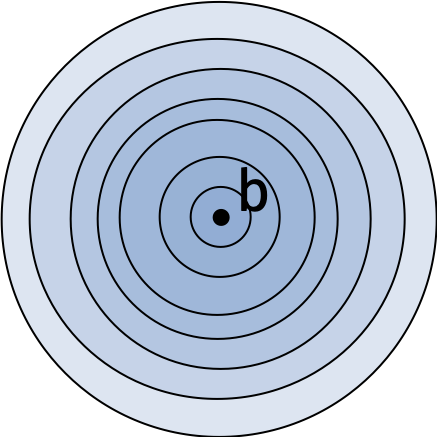
\includegraphics[width=.5\textwidth]{perfect_conditioning.png}
		
		Level sets of $\|\bv{D}\bv{x} - \bv{b}\|_2^2$ when $d_1^2 = 1, d_2^2 = 1$. 
	\end{center}
\end{frame}

\begin{frame}[t]
	\frametitle{geometric view}
	\begin{center}
		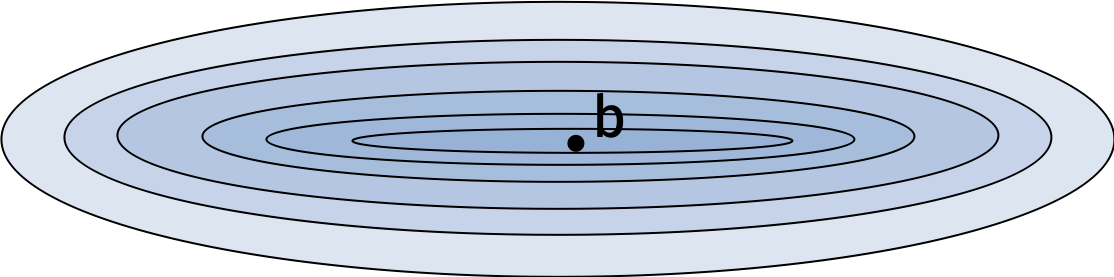
\includegraphics[width=\textwidth]{poor_conditioning.png}
		
		Level sets of $\|\bv{D}\bv{x} - \bv{b}\|_2^2$ when $d_1^2 = \frac{1}{3}, d_2^2 = 2$. 
	\end{center}

\vspace{8em}
What about non-diagonal $\bv{D}$?
\end{frame}

\begin{frame}[t]
	\frametitle{eigendecomposition view}
	Any symmetric matrix $\bv{H}$ has an \emph{orthogonal}, real valued eigendecomposition. 
	\begin{center}
		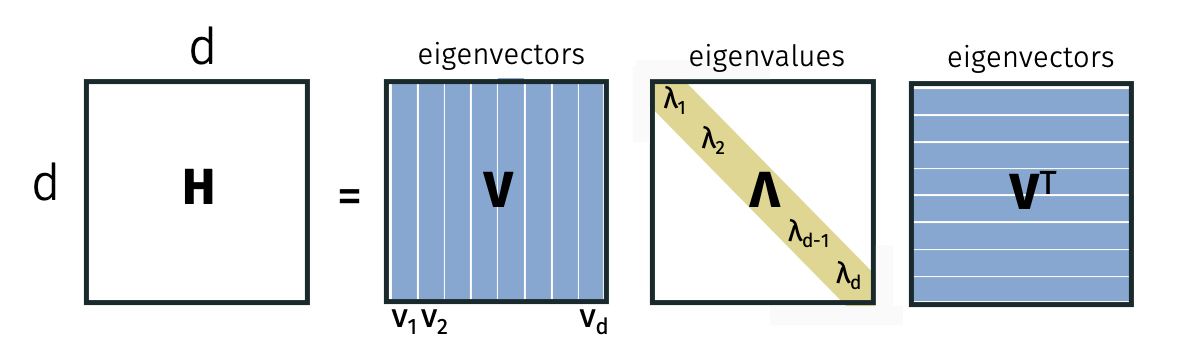
\includegraphics[width=.9\textwidth]{eigendecomp.png}
	\end{center}
	Here $\bv{V}$ is square and orthogonal, so $\bv{V}^T\bv{V} = \bv{V}\bv{V}^T = \bv{I}$. And for each $\bv{v}_i$, we have:
	\begin{align*}
		\bv{H}\bv{v}_i = \lambda_i \bv{v}_i. 
	\end{align*}
	By definition, that's what makes $\bv{v}_1, \ldots, \bv{v}_d$ eigenvectors.	
\end{frame}

\begin{frame}[t]
	\frametitle{eigendecomposition view}
	Recall $\bv{V}\bv{V}^T = \bv{V}^T\bv{V} = \bv{I}$.
	\begin{center}
		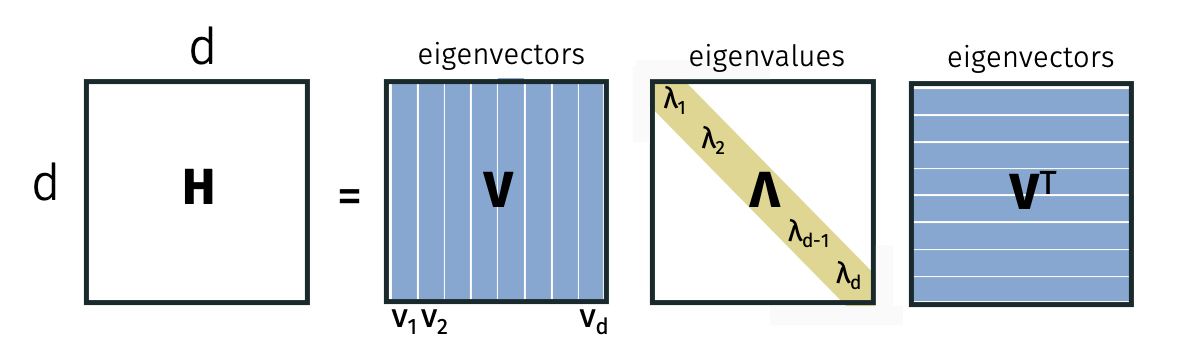
\includegraphics[width=.9\textwidth]{eigendecomp.png}
	\end{center}
	\textbf{Claim:}	$\bv{H} \text{ is PSD } \Leftrightarrow \lambda_1, ..., \lambda_d \geq 0$. 
\end{frame}

\begin{frame}[t]
	\frametitle{eigendecomposition view}
	Recall $\bv{V}\bv{V}^T = \bv{V}^T\bv{V} = \bv{I}$.
	\begin{center}
		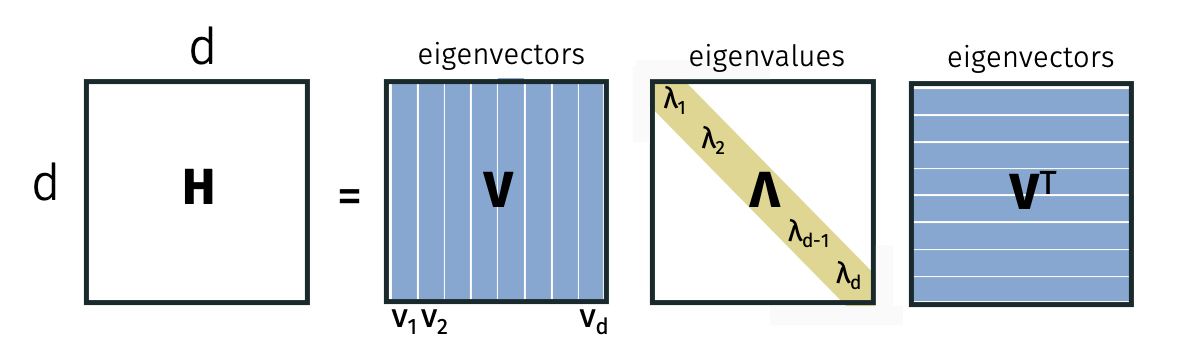
\includegraphics[width=.9\textwidth]{eigendecomp.png}
	\end{center}
	\textbf{Claim:}	$\alpha\bv{I} \preceq \bv{H} \preceq \beta \bv{I} \Leftrightarrow \alpha \leq \lambda_d \leq ... \leq \lambda_1 \leq \beta$. 
\end{frame}

\begin{frame}[t]
	\frametitle{eigendecomposition view}
	Recall $\bv{V}\bv{V}^T = \bv{V}^T\bv{V} = \bv{I}$.
	\begin{center}
		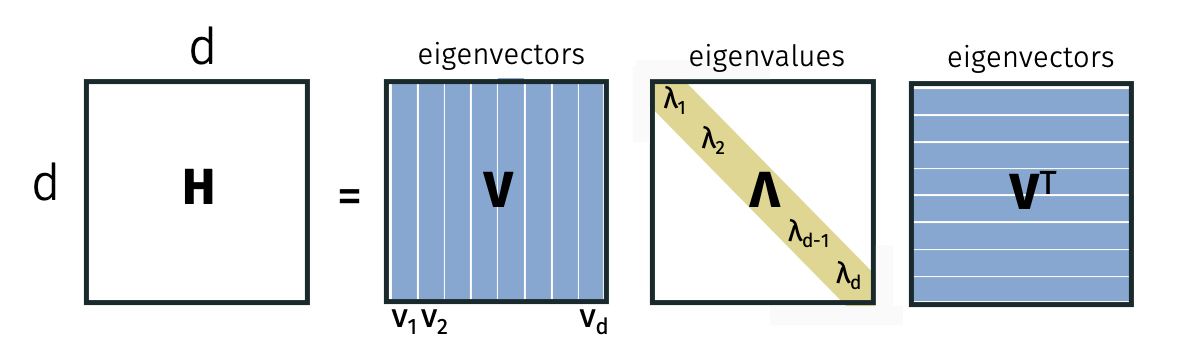
\includegraphics[width=.9\textwidth]{eigendecomp.png}
	\end{center}
	In other words, if we let $\lmax(\bv{H})$ and $\lmin(\bv{H})$ be the smallest and largest eigenvalues of $\bv{H}$, then for all $\bv{z}$ we have: 
	\begin{align*}
		\bv{z}^T\bv{H}\bv{z} &\leq \lmax(\bv{H})\cdot \|\bv{z}\|^2 \\
		\bv{z}^T\bv{H}\bv{z} &\geq \lmin(\bv{H})\cdot \|\bv{z}\|^2 
	\end{align*}
	
\end{frame}


\begin{frame}[t]
	\frametitle{eigendecomposition view}
	If the maximum eigenvalue of $\bv{H} = \nabla^2f(\bv{x}) = \beta$ and the minimum eigenvalue of $\bv{H} = \nabla^2f(\bv{x}) = \alpha$ then $f(\bv{x})$ is $\beta$-smooth and $\alpha$-strongly convex.
	
	\begin{align*}
		\lmax(\bv{H}) &= \beta\\
		\lmin(\bv{H}) &= \alpha
	\end{align*}
\end{frame}

\begin{frame}[t]
	\frametitle{polynomial view point}
	\begin{theorem}[GD for $\beta$-smooth, $\alpha$-strongly convex.]
		Let $f$ be a $\beta$-smooth and $\alpha$-strongly convex function. If we run GD for $S$ steps (with step size $\eta = \frac{1}{\beta}$) we have:
		\begin{align*}
			\|\bv{x}^{(S)} - \bv{x}^*\|_2 \leq e^{-S/\kappa} \|\bv{x}^{(0)} - \bv{x}^*\|_2
		\end{align*} 
	\end{theorem}
	
	\begin{center}
		\alert{\textbf{Goal: Prove for $f(\bv{x}) = \|\bv{A}\bv{x} - \bv{b}\|_2^2$.}}
	\end{center}	
	Let $\lmax = \lmax(\bv{A}^T\bv{A})$ and set step size $\eta = \frac{1}{2\lambda_{max}}$. Gradient descent update is:
	\begin{align*}
		\bv{x}^{(t+1)} = \bv{x}^{(t)} - \frac{1}{2\lmax}2\bv{A}^T(\bv{A}\bv{x}^{(t)} - \bv{b})
	\end{align*}
	
\end{frame}

\begin{frame}[t]
	\frametitle{alternative view of gradient descent}
	\textbf{Richardson Iteration view:}
	\begin{align*}
		(\bv{x}^{(t+1)} - \bv{x}^*) =  \left(\bv{I} - \frac{1}{\lmax}\bv{A}^T\bv{A}\right)(\bv{x}^{(t)} - \bv{x}^*) 
	\end{align*}
	


\end{frame}

\begin{frame}[t]
	\frametitle{unrolled gradient descent}
	\begin{align*}
		(\bv{x}^{(S)} - \bv{x}^*) =  \left(\bv{I} - \frac{1}{\lmax}\bv{A}^T\bv{A}\right)^S(\bv{x}^{(0)} - \bv{x}^*) 
	\end{align*}
	

\end{frame}

\begin{frame}[t]
	\frametitle{unrolled gradient descent}
	\begin{align*}
		(\bv{x}^{(S)} - \bv{x}^*) =  \left(\bv{I} - \frac{1}{\lmax}\bv{A}^T\bv{A}\right)^S(\bv{x}^{(0)} - \bv{x}^*) 
	\end{align*}
	
	\textbf{Approach:} Show that the maximum eigenvalue of $\left(\bv{I} - \frac{1}{\lmax}\bv{A}^{T}\bv{A}\right)^{2S}$ is small -- i.e., bounded by $e^{-S/\kappa} = \epsilon$. 
	
	\textbf{Conclusion:}
	 $\|\bv{x}^{(S)} - \bv{x}^*\|_2^2 \leq $
	
	So we have $\|\bv{x}^{(S)} - \bv{x}^*\|_2 \leq $
\end{frame}

\begin{frame}[t]
	\frametitle{unrolled gradient descent}
	\begin{align*}
		(\bv{x}^{(S)} - \bv{x}^*) =  \left(\bv{I} - \frac{1}{\lmax}\bv{A}^T\bv{A}\right)^S(\bv{x}^{(0)} - \bv{x}^*) 
	\end{align*}

	What is the maximum eigenvalue of the symmetric matrix $\left(\bv{I} - \frac{1}{\lmax}\bv{A}^T\bv{A}\right)$ in terms of the eigenvalues of $\bv{A}^T\bv{A}$?
	
\end{frame}

\begin{frame}[t]
	\frametitle{unrolled gradient descent}
	\begin{align*}
		(\bv{x}^{(S)} - \bv{x}^*) =  \left(\bv{I} - \frac{1}{\lmax}\bv{A}^T\bv{A}\right)^S(\bv{x}^{(0)} - \bv{x}^*) 
	\end{align*}
	
	What is the maximum eigenvalue of $\left(\bv{I} - \frac{1}{\lmax}\bv{A}^T\bv{A}\right)^S$?
	
	
\end{frame}



%\begin{frame}
%	\frametitle{improving gradient descent}
%	We now have a pretty good understanding of gradient descent. 
%	
%	\textbf{Number of iterations for $\epsilon$ error:}
%	\begin{center}
%		\begin{tabular}{c|cc}
%			& $G$-Lipschitz & $\beta$-smooth   \\ \hline
%			$R$ bounded start & $O\left(\frac{G^2R^2}{\epsilon^2}\right)$ & $O\left(\frac{\beta R^2}{\epsilon}\right)$ \\
%			$\alpha$-strong convex & $O\left(\frac{G^2}{\alpha\epsilon}\right)$ & $O\left(\frac{\beta}{\alpha}\log(1/\epsilon)\right)$
%		\end{tabular}
%	\end{center}
%	
%	%	\vspace{1em}
%	%	\alert{How do we use this understanding to design \emph{faster algorithms?}}
%\end{frame}

\begin{frame}[standout]
	\begin{center}
		\large acceleration
	\end{center}
\end{frame}


\begin{frame}
	\frametitle{accelerated gradient descent}
	\textbf{Nesterov's accelerated gradient descent}:
	\begin{itemize}
		\item $\bv{x}^{(0)} = \bv{y}^{(1)} = \bv{z}^{(1)}$  
		\item For $t = 1,\ldots, T$
		\begin{itemize}
			\item $\bv{y}^{(t+1)} = \bv{x}^{(t)} - \frac{1}{\beta}\nabla f(\bv{x}^{(t)})$
			\item $\bv{x}^{(t+1)} = \left(1 + \frac{\sqrt{\kappa} - 1}{\sqrt{\kappa} + 1}\right) \bv{y}^{(t+1)} + \frac{\sqrt{\kappa} - 1}{\sqrt{\kappa} + 1}\left(\bv{y}^{(t+1)} - \bv{y}^{(t)}\right)$
		\end{itemize}
	\end{itemize}
	\begin{theorem}[AGD for $\beta$-smooth, $\alpha$-strongly convex.]
		Let $f$ be a $\beta$-smooth and $\alpha$-strongly convex function. If we run AGD for $S$ steps we have:
		\begin{align*}
			f(\bv{x}^{(S)}) - f(\bv{x}^*) \leq \kappa e^{-S/\sqrt{\kappa}} \left[f(\bv{x}^{(0)}) - f(\bv{x}^*) \right]
		\end{align*} 
	\end{theorem}	
	\textbf{Corollary:} If \alert{$T = O\left(\sqrt{\kappa}\log(\kappa/\epsilon)\right)$ achieve error $\epsilon$.} 
	
\end{frame}
%
%\begin{frame}[t]
%	\frametitle{linear regression runtime}
%	\textbf{Total runtime for solving linear regression via GD}:
%	\begin{center}
%		(time per iteration) x (number of iterations)
%		
%		\vspace{5em}
%		
%		\large
%		$\alert{O(nd\cdot\kappa\log(1/\epsilon))}$
%		
%		for $\bv{A}\in \R^{n\times d}$, $\bv{x} \in \R^d$, $\bv{b}\in \R^n$.
%	\end{center}	
%\end{frame}
%
%\begin{frame}[t]
%	\frametitle{acceleration}
%	\begin{theorem}[Accelerated Iterative Regression]
%		Let $\bv{x}^* = \min_{\bv{x}}\|\bv{A}\bv{x} - \bv{b}\|_2^2$. There is an algorithm which finds $\tilde{\bv{x}} $ with $\|\tilde{\bv{x}} - \bv{x}^*\|_2 \leq \epsilon\|\bv{x}^*\|_2$ in time:
%			\begin{align*}
%				O(nd\cdot\sqrt{\kappa\log(1/\epsilon)})
%			\end{align*} 
%	\end{theorem}
%\end{frame}
%
%\begin{frame}[t]
%	\frametitle{the polynomial view}
%	\textbf{Claim:} For any $\eta$, polynomial $p(z) = c_1 z + c_2 z^2 + \ldots + c_q z^q$ with $p(1) = \sum_{j=1}^q c_q = 1$, there is an algorithm running in $O(ndq)$ time which outputs $\tilde{\bv{x}}$ satisfying:
%	\begin{align*}
%	\tilde{\bv{x}} - \bv{x}^* =  p(\bv{I} - \frac{1}{\eta}\bv{A}^T\bv{A}) \bv{x}^*
%	\end{align*}
%	
%	\begin{center}
%		\alert{For standard gradient descent, $p(z) = z^q$.}
%	\end{center}
%\end{frame}
%
%\begin{frame}[t]
%	\frametitle{the polynomial view}
%	\textbf{Claim:} For any $\eta$, polynomial $p(z) = c_1 z + c_2 z^2 + \ldots + c_q z^q$ with $p(1) = \sum_{j=1}^q c_q = 1$, there is an algorithm running in $O(ndq)$ time which outputs $\tilde{\bv{x}}$ satisfying:
%	\begin{align*}
%	\tilde{\bv{x}} - \bv{x}^* =  c_1\cdot (\bv{I} - \eta\bv{A}^T\bv{A})\bv{x}^* + c_2 \cdot (\bv{I} - \eta\bv{A}^T\bv{A})^2  \bv{x}^* + \ldots + c_q \cdot (\bv{I} - \eta\bv{A}^T\bv{A})^q  \bv{x}^* 
%	\end{align*}
%	
%	\textbf{Claim:} $c_j  \cdot \bv{I} - \eta\bv{A}^T\bv{A})^j\bv{x}^* = c_j\cdot\bv{x}^* + p_j'(\bv{I} - \eta\bv{A}^T\bv{A})\bv{A}^T\bv{A}\bv{x}^*$ where $p_j$ is a polynomial with degree $j - 1$.
%\end{frame}
%
%\begin{frame}[t]
%	\frametitle{the polynomial view}
%	\textbf{Claim:} For any $\eta$, polynomial $p(z) = c_1 z + c_2 z^2 + \ldots + c_q z^q$ with $p(1) = \sum_{j=1}^q c_q = 1$, there is an algorithm running in $O(ndq)$ time which outputs $\tilde{\bv{x}}$ satisfying:
%	\begin{align*}
%	\bv{x}^* - \tilde{\bv{x}} &=  (c_1 + c_2 + \ldots + c_q)\cdot\bv{x}^* +  p'(\bv{I} - \eta\bv{A}^T\bv{A})\bv{A}^T\bv{A}\bv{x}^*
%	\end{align*}
%	\begin{align*}
%		\tilde{\bv{x}}  &= p'(\bv{I} - \eta\bv{A}^T\bv{A})\bv{A}^T\bv{b} \text{ where $p'$ is a polynmial with degree $q-1$}.
%	\end{align*}
%\end{frame}
%
%\begin{frame}[t]
%	\frametitle{the polynomial view}
%	\begin{align*}
%	\tilde{\bv{x}} - \bv{x}^* =  p(\bv{I} - \eta\bv{A}^T\bv{A})\bv{x}^*\\
%	p(\bv{I} - \eta\bv{A}^T\bv{A}) = \bv{U}p(\bv{I} - \eta\bs{\Lambda})\bv{U}^T
%	\end{align*}
%	
%	\begin{align*}
%	\|\tilde{\bv{x}} - \bv{x}^*\|  &= \|\bv{U}p(\bv{I} - \eta\bs{\Lambda})\bv{U}^T\bv{x}^*\|_2 \\
%	& = \|p(\bv{I} - \eta\bs{\Lambda})\bv{U}^T\bv{x}^*\|_2
%	\end{align*}
%	
%	As long as $\max\left[ p(\bv{I} - \eta\bs{\Lambda})\right] \leq \epsilon$, 
%	\begin{align*}
%	\|\tilde{\bv{x}} - \bv{x}^*\|_2  \leq \epsilon \|\bv{x}^*\|_2 
%	\end{align*}
%\end{frame}
%
%\begin{frame}[t]
%	\frametitle{constructing a jump polynomial}
%	\textbf{Goal:} Find polynomial $p$ such that $p(1) = 1$ and $p(z) \leq \epsilon$ for $z\in [0,1 - \frac{1}{\kappa}]$.
%	\begin{center}
%		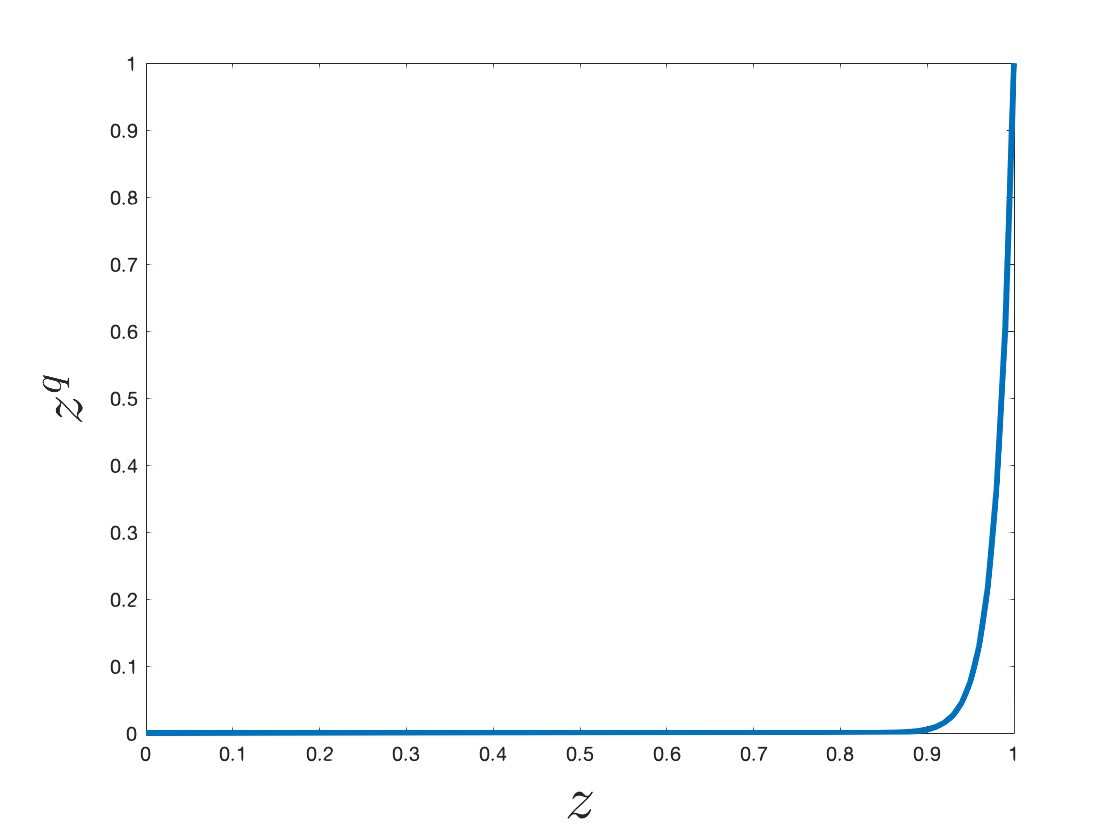
\includegraphics[width=.6\textwidth]{basic_jump.png}
%		
%		Gradient descent uses $p(z) = z^{O(\kappa\log(1/\epsilon))}$.
%	\end{center}
%\end{frame}
%
%\begin{frame}[t]
%	\frametitle{a better jump polynomial}
%		\textbf{Goal:} Find polynomial $p$ such that $p(1) = 1$ and $p(z) \leq \epsilon$ for $z\in [0,1 - \frac{1}{\kappa}]$.
%	\begin{center}
%		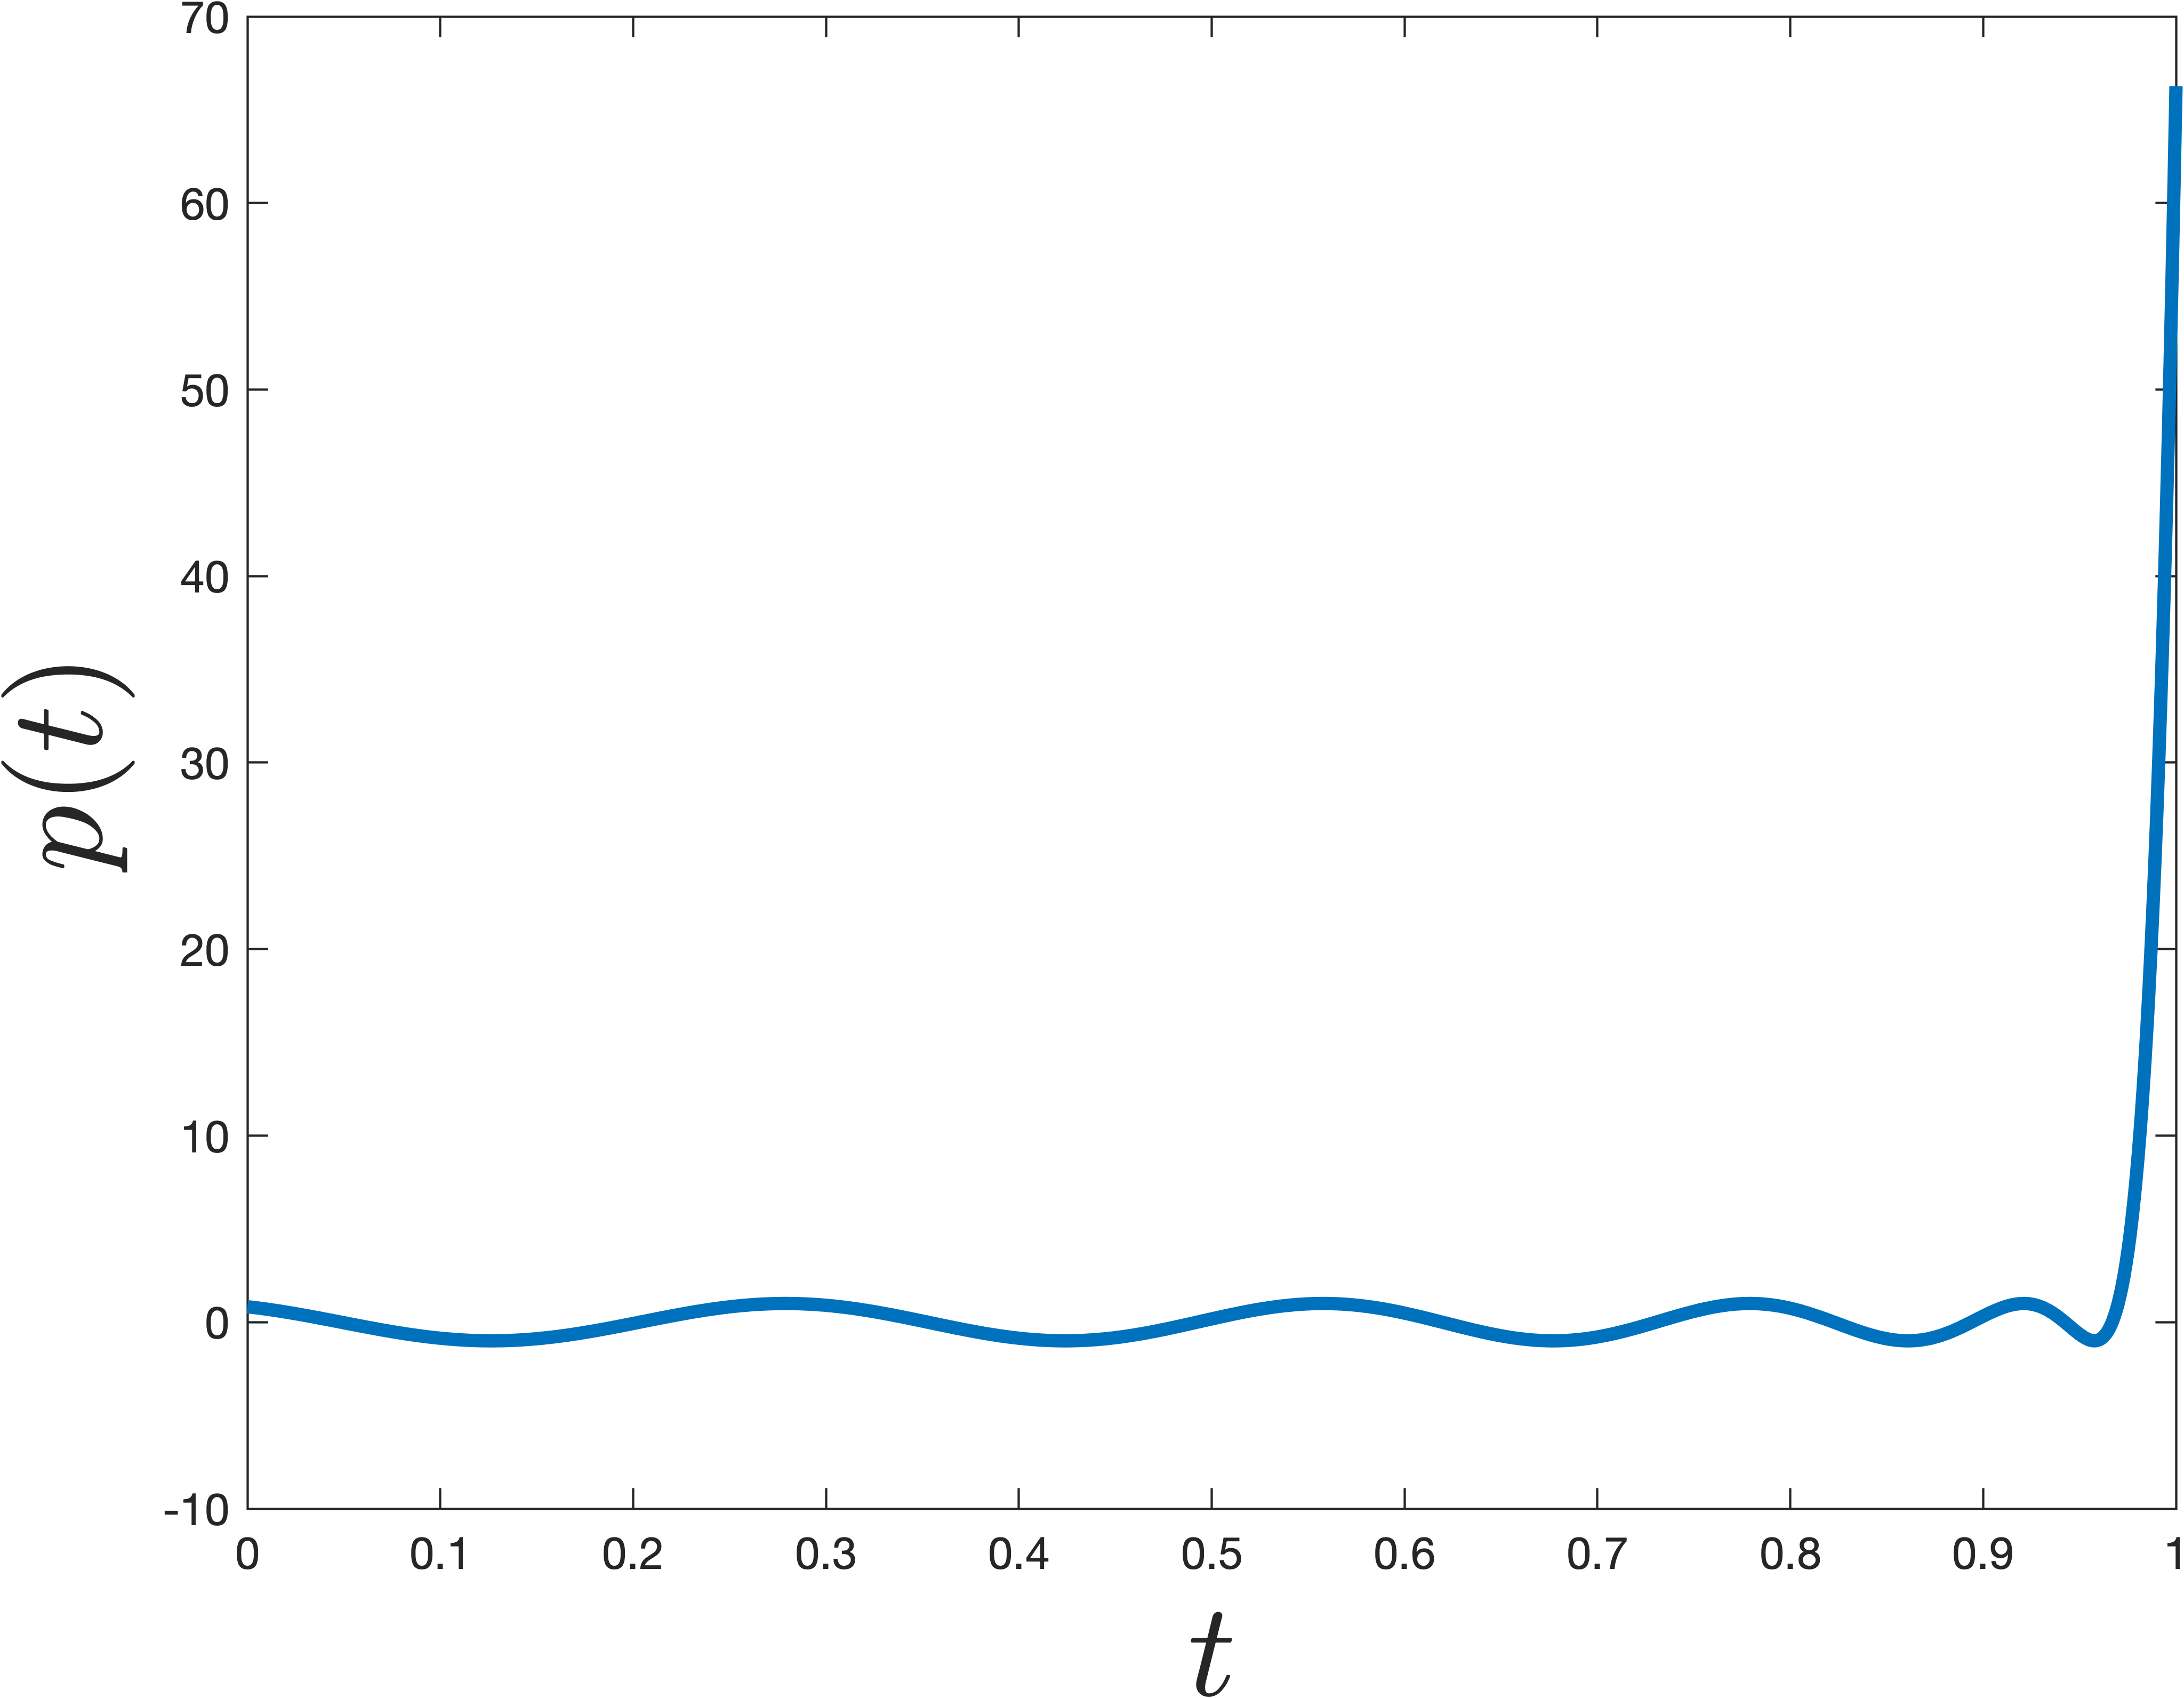
\includegraphics[width=.6\textwidth]{cheby_jump.png}
%		
%		\alert{Can be done with degree $O(\sqrt{\kappa\log(1/\epsilon)})$ polynomial instead!}
%	\end{center}
%\end{frame}
%
%\begin{frame}
%	\frametitle{chebyshev polynomials}
%	\begin{center}
%		\textbf{What are these polynomials?}
%	\end{center}
%	
%		\centering
%		Chebyshev polynomials of the first kind.
%		\begin{columns}
%			\begin{column}{0.5\textwidth}
%				\begin{align*}
%				T_0(x) &= 1\\
%				T_1(x) &= x \\
%				T_2(x) &= 2x^2 - 1\\
%				&\,\,\,\vdots\\
%				T_k(x) &= 2xT_{k-1}(x) - T_{k-2}(x)\\
%				\end{align*}
%			\end{column}
%			\begin{column}{0.5\textwidth}
%				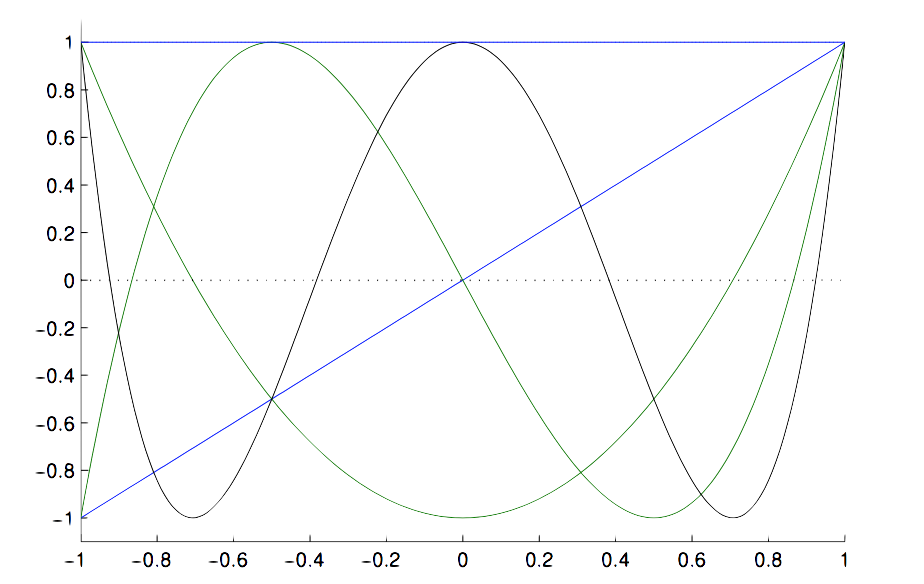
\includegraphics[width=\textwidth]{chebyPolys.png}
%			\end{column}
%		\end{columns}
%		\begin{center}
%			\textbf{``There's only one bullet in the gun. It's called the Chebyshev polynomial.''} -- Prof. Rocco Servedio
%		\end{center}
%\end{frame}
%
%\begin{frame}
%	\frametitle{accelerated gradient descent}
%	\textbf{Nesterov's accelerated gradient descent}:
%	\begin{itemize}
%		\item $\bv{x}^{(0)} = \bv{y}^{(1)} = \bv{z}^{(1)}$  
%		\item For $t = 1,\ldots, T$
%		\begin{itemize}
%			\item $\bv{y}^{(t+1)} = \bv{x}^{(t)} - \frac{1}{\beta}\nabla f(\bv{x}^{(t)})$
%			\item $\bv{x}^{(t+1)} = \left(1 + \frac{\sqrt{\kappa} - 1}{\sqrt{\kappa} + 1}\right) \bv{y}^{(t+1)} - \frac{\sqrt{\kappa} - 1}{\sqrt{\kappa} + 1}\bv{y}^{(t)}$
%		\end{itemize}
%	\end{itemize}
%	\begin{theorem}[AGD for $\beta$-smooth, $\alpha$-strongly convex.]
%	Let $f$ be a $\beta$-smooth and $\alpha$-strongly convex function. If we run AGD for $T$ steps we have:
%	\begin{align*}
%	f(\bv{x}^{(t)}) - f(\bv{x}^*) \leq \kappa e^{-(t-1)\sqrt{\kappa}} \left[f(\bv{x}^{(0)}) - f(\bv{x}^*) \right]
%	\end{align*} 
%\end{theorem}	
%\textbf{Corollary:} If \alert{$T = O\left(\sqrt{\kappa}\log(\kappa/\epsilon)\right)$ achieve error $\epsilon$.} 
%	
%\end{frame}

\begin{frame}[t]
	\frametitle{intuition behind acceleration}
	\begin{center}
		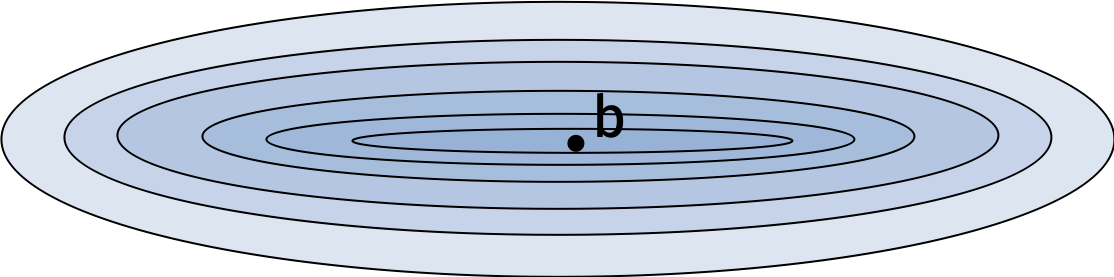
\includegraphics[width=\textwidth]{poor_conditioning.png}
		
		Level sets of $\|\bv{A}\bv{x} - \bv{b}\|_2^2$.
	\end{center}
	
	\textbf{Other terms for similar ideas:}
	\begin{itemize}
		\item Momentum
		\item Heavy-ball methods
	\end{itemize}
	
	\begin{center}
		\alert{What if we look back beyond \emph{two iterates}?}
	\end{center}
\end{frame}


\begin{frame}[standout]
	\begin{center}
		break
	\end{center}
\end{frame}


\begin{frame}[t]
	\frametitle{online and stochastic gradient descent}
	\textbf{Second part of class:}
	\begin{itemize}
		\item Basics of \emph{Online Learning + Optimization}. 
		\item Introduction to \emph{Regret Analysis}.
		\item Application to analyzing \emph{Stochastic Gradient Descent.}
	\end{itemize}
	
\end{frame}


\begin{frame}
	\frametitle{online learning}
	\begin{center}
		\textbf{Many machine learning problems are solved in an \emph{online} setting with constantly changing data.}
	\end{center}
	\begin{itemize}
		\item Spam filters are incrementally updated and adapt as they see more examples of spam over time. 
		\item Image classification systems learn from mistakes over time (often based on user feedback). 
		\item Content recommendation systems adapt to user behavior and clicks (which may not be a good thing...)
	\end{itemize}
\end{frame}


\begin{frame}
	\frametitle{example}
	\begin{center}
	\textbf{Plant identification via iNaturalist app.}
		
	(California Academy of Science + National Geographic)
	\end{center}
\begin{columns}
	\begin{column}{.5\textwidth}
		\centering
		
\includegraphics[width=.5\textwidth]{inaturalist.png}
	\end{column}
	\begin{column}{.5\textwidth}
		\begin{itemize}
			\item When the app fails, image is classified via crowdsourcing (backed by huge network of amateurs and experts).
		
			\item Single model that is updated constantly, not retrained in batches.
		\end{itemize}
	\end{column}
\end{columns}
\end{frame}

\begin{frame}
	\frametitle{example}
		\begin{center}
		\textbf{ML based email spam/scam filtering.}
	\end{center}
	\begin{center}
		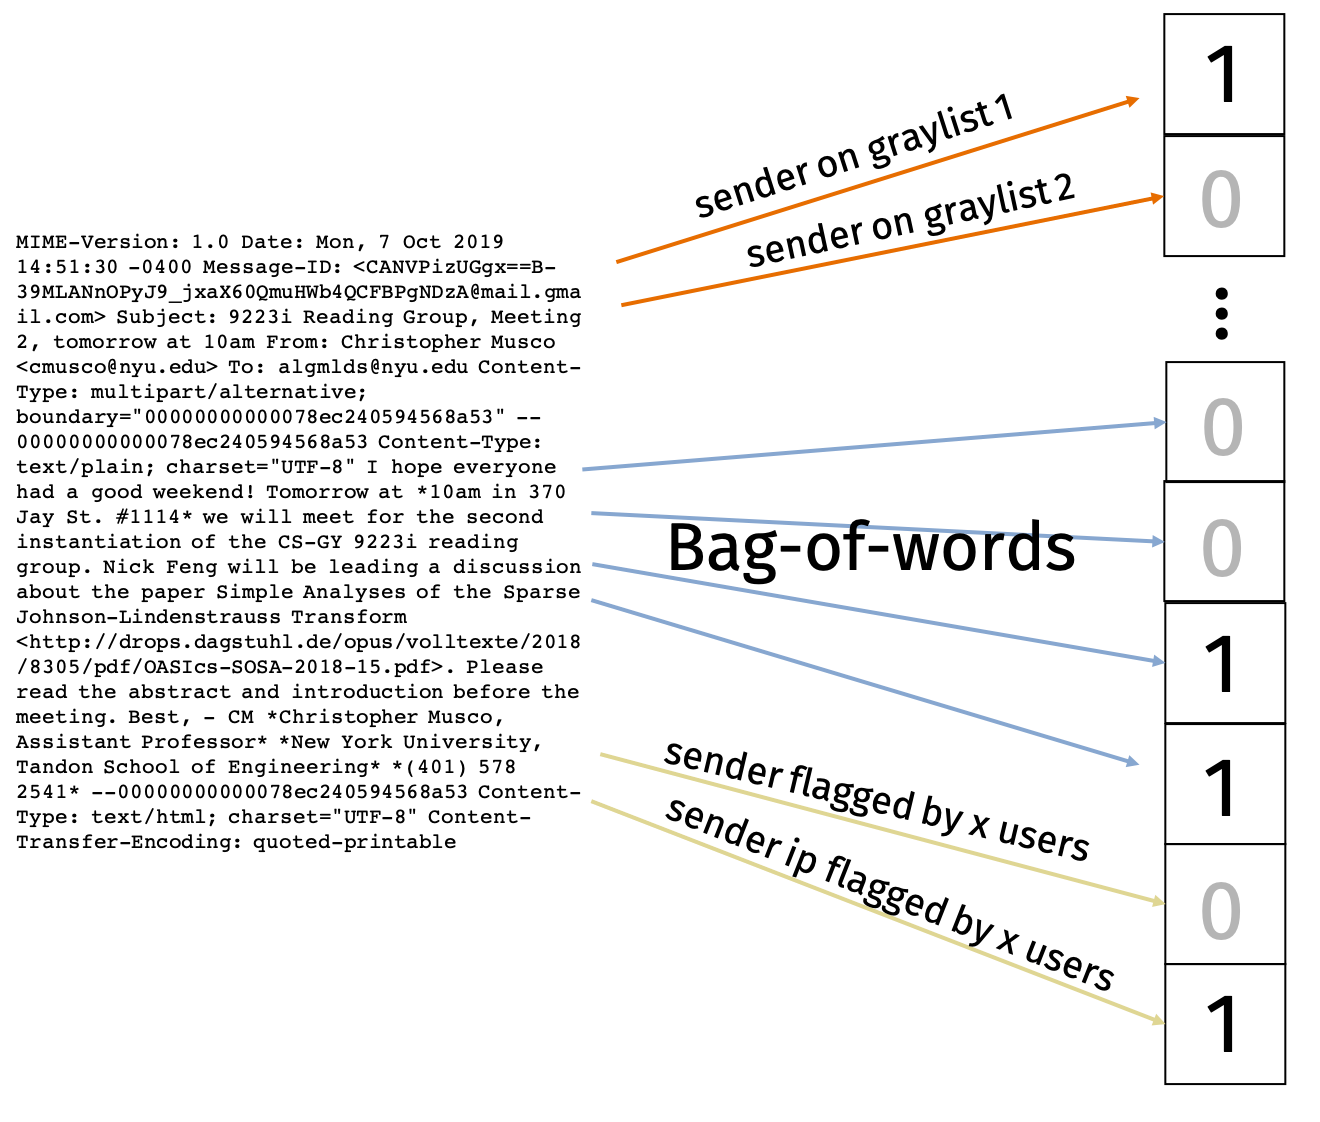
\includegraphics[width=.5\textwidth]{spam_features.png}
	\end{center}
Markers for spam change overtime, so model might change.
\end{frame}

\begin{frame}
	\frametitle{example}
	\begin{center}
		\textbf{ML based email spam/scam filtering.}
	\end{center}
	\begin{center}
		
\includegraphics[width=.4\textwidth]{covid_spam.png}
	\end{center}
	Markers for spam change overtime, so model might change.
\end{frame}

\begin{frame}
	\frametitle{online learning framework}
	Choose some model $M_\bv{x}$ parameterized by parameters $\bv{x}$ and some loss function $\ell$. 
	At time steps $1,\ldots, T$, receive data vectors $\bv{a}^{(1)}, \ldots, \bv{a}^{(T)}$. 
	\begin{itemize}
		\item At each time step, we pick (``play'') a parameter vector $\bv{x}^{(i)}$.
		\item Make prediction $\tilde{y}^{(i)} = M_{\bv{x}^{(i)}}(\bv{a}_i)$.
		\item Then told true value or label $y^{(i)}$. 
		\item Goal is to minimize cumulative loss:
		\begin{align*}
			L = \sum_{i=1}^n \ell(\bv{x}^{(i)}, \bv{a}^{(i)}, y^{(i)})
		\end{align*} 
	\end{itemize}
	For example, for a regression problem we might use the $\ell_2$ loss:
	\begin{align*}
		\ell(\bv{x}^{(i)}, \bv{a}^{(i)}, y^{(i)}) = \left|\langle\bv{x}^{(i)},\bv{a}^{(i)}\rangle - y^{(i)}\right|^2. 
	\end{align*}
For classification, we could use logistic/cross-entropy loss. 
\end{frame}

\begin{frame}
	\frametitle{online optimization}
	\textbf{Abstraction as optimization problem:} Instead of a single objective function $f$, we have a single (initially unknown) function $f_1, \ldots, f_T: \R^d \rightarrow \R$ for each time step. 
	\begin{itemize}
		\item For time step $i\in 1,\ldots, T$, select vector $\bv{x}^{(i)}$.
		\item Observe $f_i$ and pay cost $f_i(\bv{x}^{(i)})$
		\item Goal is to minimize $\sum_{i=1}^T f_i(\bv{x}^{(i)})$. 
	\end{itemize}

	\begin{center}
		We make \emph{no assumptions} that $f_1, \ldots, f_T$ are related to each other at all!
	\end{center}
\end{frame}

\begin{frame}[t]
	\frametitle{regret bound}
	In offline optimization, we wanted to find $\hat{\bv{x}}$ satisfying $f(\hat{\bv{x}}) \leq \min_{\bv{x}} f(\bv{x})$. Ask for a similar thing here. 
	
	\textbf{Objective:} Choose $\bv{x}^{(0)}, \ldots, \bv{x}^{(T)}$ so that: 
	\begin{align*}
		\sum_{i=1}^T f_i(\bv{x}^{(i)}) \leq \left[\min_\bv{x} \sum_{i=1}^T f_i(\bv{x})\right] + \epsilon.
	\end{align*}
	Here $\alert{\epsilon}$ is called the \alert{\textbf{regret}} of our solution sequence $\bv{x}^{(0)}, \ldots, \bv{x}^{(T)}$.
	
	We typically $\epsilon$ to be growing \emph{sublinearly} in $T$. 
\end{frame}

\begin{frame}[t]
	\frametitle{regret bound}
	\begin{center}
		Regret compares to the best \emph{fixed} solution in hindsight.
	\end{center}
	\begin{align*}
		\sum_{i=1}^T f_i(\bv{x}^{(i)}) \leq \left[\min_\bv{x} \sum_{i=1}^T f_i(\bv{x})\right] + \epsilon.
	\end{align*}
	It's very possible that $\sum_{i=1}^T f_i(\bv{x}^{(i)}) < \left[\min_\bv{x} \sum_{i=1}^T f_i(\bv{x})\right]$. Could we hope for something stronger?
	
	\textbf{Exercise:} Argue that the following is impossible to achieve:
	\begin{align*}
		\sum_{i=1}^T f_i(\bv{x}^{(i)}) \leq \left[\sum_{i=1}^T \min_\bv{x} f_i(\bv{x})\right] + \epsilon.
	\end{align*}
\end{frame}

\begin{frame}[t]
	\frametitle{hard example for online optimization}
	\textbf{Convex functions:}
	\begin{align*}
		f_1(x) &= |x - h_1|\\
		 &\vdots\\
		 f_n(x) &= |x - h_T|
	\end{align*}
where $h_1, \ldots, h_T$ are i.i.d. uniform $\{0,1\}$.
\end{frame}

\begin{frame}[t]
	\frametitle{regret bounds}
	\begin{align*}
		\sum_{i=1}^T f_i(\bv{x}^{(i)}) \leq \left[\min_\bv{x} \sum_{i=1}^T f_i(\bv{x})\right] + \epsilon.
	\end{align*}
	
	\textbf{Beautiful balance:}
	\begin{itemize}
		\item Either $f_1, \ldots, f_T$ are similar or changing slowly, so we can learn predict $f_i$ from earlier functions.
		\item Or $f_1, \ldots, f_T$  are very different, in which case $\min_\bv{x} \sum_{i=1}^T f_i(\bv{x})$ is large, so regret bound is easy to achieve. 
		\item Or we live somewhere in the middle.
	\end{itemize} 
\end{frame}

\begin{frame}[t]
	\frametitle{follow-the-leader}
		\textbf{Follow-the-leader algorithm:}
	\begin{itemize}
		\item Choose $\bv{x}^{(0)}$.
		\item For $i = 1,\ldots, T$:
		\begin{itemize}
			\item Let $\bv{x}^{(i)} = \argmin_{j=1}^{i-1} f_j(\bv{x})$.
			\item Play $\bv{x}^{(i)}$.
			\item Observe $f_{i}$ and incur cost $f_{i}(\bv{x}^{(i)})$. 
		\end{itemize}
	\end{itemize}
Simple and intuitive, but there are \emph{two} issues with this approach. One is computational, one is related to the accuracy.
	
\end{frame}

\begin{frame}[t]
	\frametitle{follow-the-leader}
	\textbf{Hard case:}
\begin{center}
	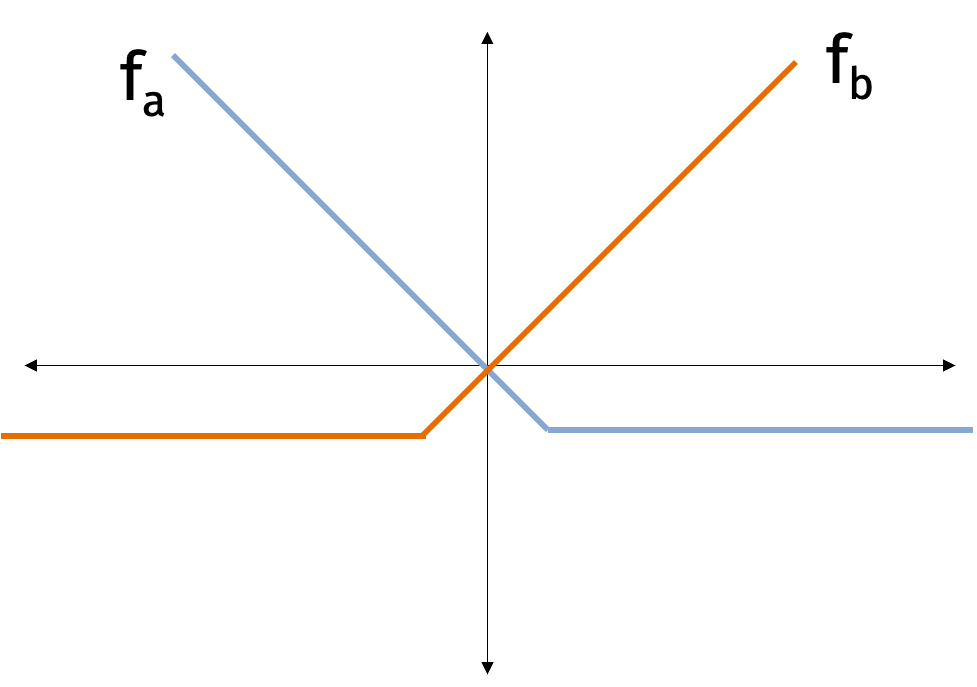
\includegraphics[width=.7\textwidth]{hard_case_ftl.png}
	\end{center}
\end{frame}


\begin{frame}[t]
	\frametitle{online gradient descent}
	\textbf{Online Gradient descent:}
\begin{itemize}
	\item Choose $\bv{x}^{(1)}$ and $\eta = \frac{R}{G\sqrt{T}}$. 
	\item For $i = 1,\ldots, T$:
	\begin{itemize}
		\item Play $\bv{x}^{(i)}$.
		\item Observe $f_{i}$ and incur cost $f_{i}(\bv{x}^{(i)})$. 
		\item $\bv{x}^{(i+1)} = \bv{x}^{(i)} - \eta \nabla f_i(\bv{x}^{(i)})$
	\end{itemize}
\end{itemize}
If $f_1, \ldots, f_T = f$ are all the same, this looks a lot like regular gradient descent. We update parameters using the gradient $\nabla f$ at each step. 
\end{frame}

\begin{frame}[t]
	\frametitle{online gradient descent (ogd)}
	$\bv{x}^{*} = \argmin_\bv{x}\sum_{i=1}^T f_i(\bv{x})$ (the offline optimum)
	
	\textbf{Assume:}
	\begin{itemize}
		\item $f_1, \ldots, f_T$ are all convex.
		\item Each is $G$-Lipschitz: for all $\bv{x}$, $i$, $\|\nabla f_i(\bv{x})\|_2 \leq \alert{G}$.
		\item Starting radius: $\|\bv{x}^{*} - \bv{x}^{(1)}\|_2 \leq \alert{R}$.
	\end{itemize}
	
	\textbf{Online Gradient descent:}
	\begin{itemize}
	\item Choose $\bv{x}^{(1)}$ and $\eta = \frac{R}{G\sqrt{T}}$. 
	\item For $i = 1,\ldots, T$:
	\begin{itemize}
		\item Play $\bv{x}^{(i)}$.
		\item Observe $f_{i}$ and incur cost $f_{i}(\bv{x}^{(i)})$. 
		\item $\bv{x}^{(i+1)} = \bv{x}^{(i)} - \eta \nabla f_i(\bv{x}^{(i)})$
	\end{itemize}
\end{itemize}
\end{frame}

\begin{frame}[t]
	\frametitle{online gradient descent analysis} 
Let $\bv{x}^{*} = \argmin_\bv{x}\sum_{i=1}^T f_i(\bv{x})$ (the offline optimum)
	\begin{theorem}[OGD Regret Bound]
		After $T$ steps, $\epsilon = \left[\sum_{i=1}^T f_i(\bv{x}^{(i)})\right] - \left[\sum_{i=1}^T f_i(\bv{x}^*)\right] \leq RG\sqrt{T}$.
	\end{theorem}
	Average regret overtime is bounded by $\frac{\epsilon}{T} \leq \frac{RG}{\sqrt{T}}$.
	
	Goes $\rightarrow 0$ as $T\rightarrow \infty$. 
	
	\begin{center}
		All this with no assumptions on how $f_1, \ldots, f_T$ relate to each other! They could have even been chosen \alert{\textbf{adversarially}} -- e.g. with $f_i$ depending on our choice of $\bv{x}_i$ and all previous choices. 
	\end{center}
\end{frame}

\begin{frame}[t]
	\frametitle{online gradient descent analysis}
	\begin{theorem}[OGD Regret Bound]
		After $T$ steps, $\epsilon = \left[\sum_{i=1}^T f_i(\bv{x}^{(i)})\right] - \left[\sum_{i=1}^T f_i(\bv{x}^*)\right] \leq RG\sqrt{T}$.
	\end{theorem}
	\textbf{Claim 1:} For all $i = 1, \ldots, T$, 
	\begin{align*}
		f_i(\bv{x}^{(i)}) - f_i(\bv{x}^*) \leq \frac{\|\bv{x}^{(i)} - \bv{x}^*\|_2^2 - \|\bv{x}^{(i+1)} - \bv{x}^*\|_2^2}{2\eta} + \frac{\eta G^2}{2}
	\end{align*}
(Same proof as last class. Only uses convexity of $f_i$.)

\end{frame}

\begin{frame}[t]
	\frametitle{online gradient descent analysis}
	\begin{theorem}[OGD Regret Bound]
		After $T$ steps, $\epsilon = \left[\sum_{i=1}^T f_i(\bv{x}^{(i)})\right] - \left[\sum_{i=1}^T f_i(\bv{x}^*)\right] \leq RG\sqrt{T}$.
	\end{theorem}
	\textbf{Claim 1:} For all $i = 1, \ldots, T$, 
	\begin{align*}
		f_i(\bv{x}^{(i)}) - f_i(\bv{x}^*) \leq \frac{\|\bv{x}^{(i)} - \bv{x}^*\|_2^2 - \|\bv{x}^{(i+1)} - \bv{x}^*\|_2^2}{2\eta} + \frac{\eta G^2}{2}
	\end{align*}
	\textbf{Telescoping Sum:} 
	\begin{align*}
		\sum_{i=1}^{T}\left[f_i(\bv{x}^{(i)}) - f_i(\bv{x}^*)\right] &\leq \frac{\|\bv{x}^{(1)}-\bv{x}^*\|_2^2 -\|\bv{x}^{(T)}-\bv{x}^*\|_2^2}{2\eta} + \frac{T\eta G^2}{2} \\ &\leq  \frac{R^2}{2\eta} + \frac{T\eta G^2}{2}
	\end{align*}
	
	
\end{frame}

\begin{frame}
	\frametitle{stochastic gradient descent (sgd)}
	Efficient \emph{offline} optimization method for functions $f$ with \emph{finite sum structure}:
	\begin{align*}
		f(\bv{x}) = \sum_{i=1}^n f_i(\bv{x}).
	\end{align*}
	
	
	Goal is to find $\hat{\bv{x}}$ such that $f(\hat{\bv{x}}) \leq f(\bv{x}^*) + \epsilon$. 
	
	\begin{itemize}
		\item The most widely use optimization algorithm in modern machine learning. 
		\item Easily analyzed as a special case of {online} gradient descent! 
	\end{itemize}
\end{frame}

\begin{frame}[t]
	\frametitle{stochastic gradient descent}
	Recall the machine learning setup. In empirical risk minimization, we can typically write:
	\begin{align*}
		f(\bv{x}) = \sum_{i=1}^n f_i(\bv{x})
	\end{align*}
	where $f_i$ is the loss function for a particular data example $(\bv{a}^{(i)},y^{(i)} )$.
	\vspace{1em}
	
	\textbf{Example: least squares linear regression.}
	\begin{align*}
		f(\bv{x}) = \sum_{i=1}^n (\bv{x}^T\bv{a}^{(i)} - y^{(i)})^2
	\end{align*}
Note that by linearity, $\nabla f(\bv{x}) = \sum_{i=1}^n \nabla f_i(\bv{x})$. 
\end{frame}

\begin{frame}
	\frametitle{stochastic gradient descent}
	{\textbf{Main idea:} Use random approximate gradient in place of actual gradient.}
	
	Pick \emph{random} $j \in 1, \ldots, n$ and update $\bv{x}$  using $\nabla f_j(\bv{x})$. 
	\begin{align*}
		\E\left[\nabla f_j(\bv{x})\right] = \frac{1}{n}\nabla f(\bv{x}).
	\end{align*}

\vspace{2em}
	$n \nabla f_j(\bv{x})$ is an unbiased estimate for the true gradient $\nabla f(\bv{x})$, but can often be computed in a $1/n$ fraction of the time!
	

	
	\begin{center}
		\alert{\textbf{Trade slower convergence for cheaper iterations.}}
	\end{center}
\end{frame}


\begin{frame}[t]
	\frametitle{stochastic gradient descent}
   {Stochastic first-order oracle} for $f(\bv{x}) = \sum_{i=1}^n f_i(\bv{x})$. 
	\begin{itemize}
		\item \textcolor{lightgray}{ \textbf{Function Query:} For any chosen $j, \bv{x}$, return $f_j(\bv{x})$}
		\item \textbf{Gradient Query:} For any chosen $j, \bv{x}$, return $\nabla f_j(\bv{x})$
	\end{itemize}
%	Computing $f(\bv{x})$ would take $n$ separate function queries. 

	\textbf{Stochastic Gradient descent:}
	\begin{itemize}
		\item Choose starting vector $\bv{x}^{(1)}$, learning rate $\eta$
		\item For $i = 1,\ldots, T$:
		\begin{itemize}
			\item Pick random $j_i \in 1, \ldots, n$.
			\item $\bv{x}^{(i+1)} = \bv{x}^{(i)} - \eta \nabla f_{j_i}(\bv{x}^{(i)})$
		\end{itemize}
		\item Return $\hat{\bv{x}} = \frac{1}{T}\sum_{i=1}^T \bv{x}^{(i)}$
	\end{itemize}
\end{frame}

\begin{frame}[t]
	\frametitle{visualizing SGD}
	\begin{center}
		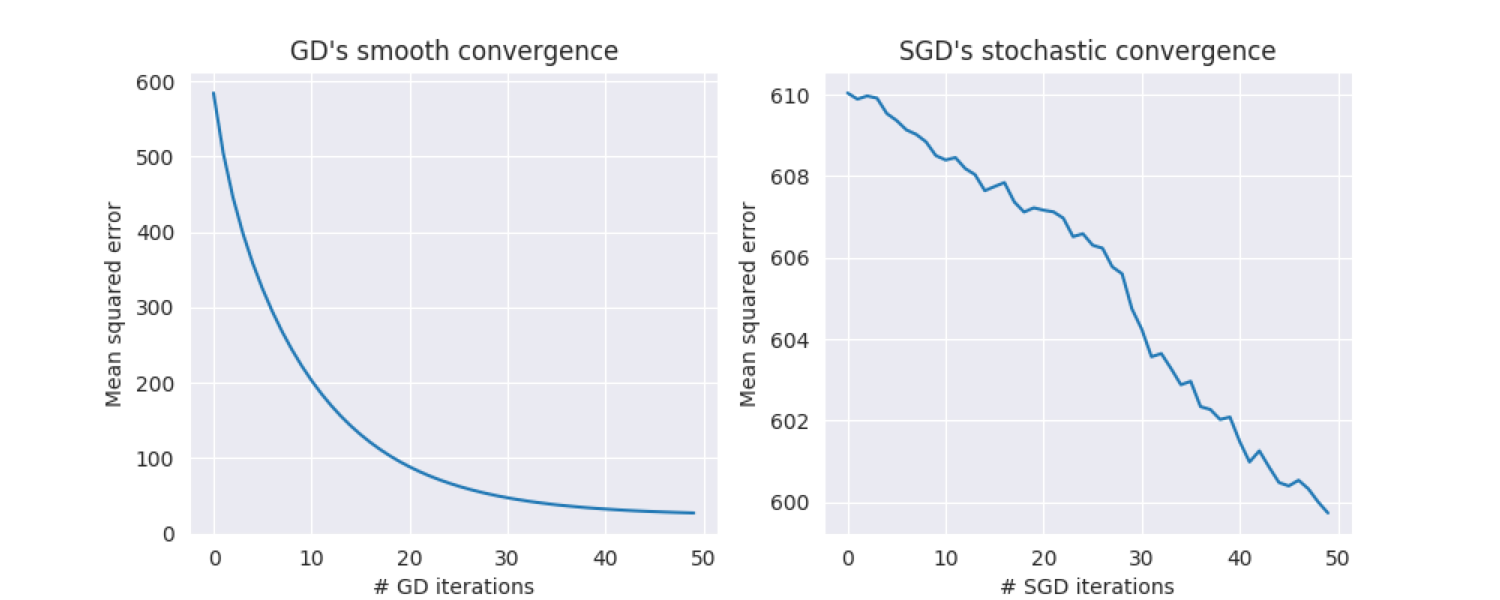
\includegraphics[height=.35\textheight]{gd_convergence.png}
		
		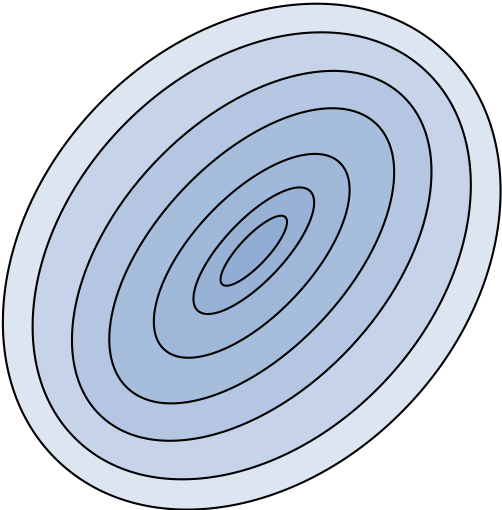
\includegraphics[height=.5\textheight]{gd_paths_raw.png}
	\end{center}	
\end{frame}


\begin{frame}[t]
	\frametitle{stochastic gradient descent}
	\small
		\vspace{-.5em}
	\textbf{Assume:}
	\vspace{-1em}
	\begin{itemize}
		\item {Finite sum structure:} $f(\bv{x}) = \sum_{i=1}^n f_i(\bv{x})$, with $f_1, \ldots, f_n$ all convex.
		\item {Lipschitz functions}: for all $\bv{x}$, $j$, $\|\nabla f_j(\bv{x})\|_2 \leq \alert{\frac{G'}{n}}$.
		\begin{itemize}
			\item What does this imply about Lipschitz constant of $f$?
		\end{itemize}
		\item Starting radius: $\|\bv{x}^{*} - \bv{x}^{(1)}\|_2 \leq \alert{R}$.
	\end{itemize}
	
	\vspace{-.5em}
	\textbf{Stochastic Gradient descent:}
	\vspace{-1em}
	\begin{itemize}
		\item Choose $\bv{x}^{(1)}$, steps $T$, learning rate $\eta = \frac{D}{G'\sqrt{T}}$.
		\item For $i = 1,\ldots, T$:
		\begin{itemize}
			\item Pick random $j_i \in 1, \ldots, n$.
			\item $\bv{x}^{(i+1)} = \bv{x}^{(i)} - \eta \nabla f_{j_i}(\bv{x}^{(i)})$
		\end{itemize}
		\item Return $\hat{\bv{x}} = \frac{1}{T}\sum_{i=1}^T \bv{x}^{(i)}$
	\end{itemize}
\alert{	\textbf{Approach: View as online gradient descent run on function sequence $f_{j_1}, \ldots, f_{j_T}$.} } 

Only use the fact that step equals gradient in expectation.
\end{frame}


\begin{frame}[t]
	\frametitle{jensen's inequality}
	For a convex function $f$ and points $\bv{x}^{(1)}, \ldots, \bv{x}^{(t)}$
	\begin{align*}
	f\left(\frac{1}{t}\cdot \bv{x}^{(1)} + \ldots + \frac{1}{t}\cdot \bv{x}^{(t)} \right) \leq \frac{1}{t}\cdot f(\bv{x}^{(1)}) + \ldots +\frac{1}{t} \cdot f(\bv{x}^{(t)} )
	\end{align*}
	
\end{frame}

\begin{frame}[t]
	\frametitle{stochastic gradient descent analysis}
	\begin{claim}[SGD Convergence]
		After $T = \frac{R^2G'^2}{\epsilon^2}$ iterations:
		\begin{align*}
			\E\left[f(\hat{\bv{x}}) - f(\bv{x}^*)\right] \leq \epsilon.
		\end{align*}

	\end{claim}
	\textbf{Claim 1:} 
	\begin{align*}
		f(\hat{\bv{x}}) - f(\bv{x}^*) \leq \frac{1}{T}\sum_{i=1}^T\left[f(\bv{x}^{(i)}) -f(\bv{x}^*)\right]
	\end{align*}
\textbf{Prove using Jensen's Inequality:}
\end{frame}

\begin{frame}[t]
	\frametitle{stochastic gradient descent analysis}
	\small
	\begin{claim}[SGD Convergence]
		After $T = \frac{R^2G'^2}{\epsilon^2}$ iterations:
		\vspace{-1em}
		\begin{align*}
			\E\left[f(\hat{\bv{x}}) - f(\bv{x}^*)\right] \leq \epsilon.
		\end{align*}
	
		\vspace{-1em}
	\end{claim}\vspace{-2em}
	\begin{align*}
		\E[f(\hat{\bv{x}}) - f(\bv{x}^*)] &\leq \frac{1}{T}\sum_{i=1}^T\E\left[f(\bv{x}^{(i)}) -f(\bv{x}^*)\right]
		\\
		&=\frac{1}{T}\sum_{i=1}^Tn\E\left[f_{j_i}(\bv{x}^{(i)}) -f_{j_i}(\bv{x}^*)\right]
	\end{align*}
\end{frame}

\begin{frame}[t]
	\frametitle{stochastic gradient descent analysis}
	\small
	\begin{claim}[SGD Convergence]
		After $T = \frac{R^2G'^2}{\epsilon^2}$ iterations:
		\vspace{-1em}
		\begin{align*}
			\E\left[f(\hat{\bv{x}}) - f(\bv{x}^*)\right] \leq \epsilon.
		\end{align*}
		
		\vspace{-1em}
	\end{claim}\vspace{-2em}
	\begin{align*}
		\E[f(\hat{\bv{x}}) - f(\bv{x}^*)] &\leq \frac{1}{T}\sum_{i=1}^T\E\left[f(\bv{x}^{(i)}) -f(\bv{x}^*)\right]
		\\
		&=\frac{1}{T}\sum_{i=1}^Tn\E\left[f_{j_i}(\bv{x}^{(i)}) -f_{j_i}(\bv{x}^*)\right]\\
		&\leq \frac{n}{T}\cdot \E\left[\sum_{i=1}^T f_{j_i}(\bv{x}^{(i)}) -f_{j_i}(\bv{x}^{offline})\right], 
	\end{align*}
where $\bv{x}^{offline} = \argmin_{\bv{x}}\sum_{i=1}^{T} f_{j_i}(\bv{x})$.
\end{frame}

\begin{frame}[t]
	\frametitle{stochastic gradient descent analysis}
	\small
	\begin{claim}[SGD Convergence]
		After $T = \frac{R^2G'^2}{\epsilon^2}$ iterations:
		\vspace{-1em}
		\begin{align*}
			\E\left[f(\hat{\bv{x}}) - f(\bv{x}^*)\right] \leq \epsilon.
		\end{align*}
		
		\vspace{-1em}
	\end{claim}\vspace{-2em}
	\begin{align*}
		\E[f(\hat{\bv{x}}) - f(\bv{x}^*)] &\leq \frac{1}{T}\sum_{i=1}^T\E\left[f(\bv{x}^{(i)}) -f(\bv{x}^*)\right]
		\\
		&=\frac{1}{T}\sum_{i=1}^Tn\E\left[f_{j_i}(\bv{x}^{(i)}) -f_{j_i}(\bv{x}^*)\right]\\
		&\leq=\frac{n}{T}\E\left[\sum_{i=1}^T f_{j_i}(\bv{x}^{(i)}) -f_{j_i}(\bv{x}^{offline})\right]\\
		& \leq \frac{n}{T} \cdot\left(R\cdot\frac{G'}{n}\cdot \sqrt{T}\right) \text{\hspace{2em} (by OGD guarantee.)}
	\end{align*}
\end{frame}


\begin{frame}[t]
	\frametitle{stochastic vs. full batch gradient descent}
	Number of iterations for error $\epsilon$:
	\begin{itemize}
		\item \textbf{Gradient Descent}: $T = \frac{R^2 G^2}{\epsilon^2}$. 
		\item \textbf{Stochastic Gradient Descent}: $T = \frac{R^2 G'^2}{\epsilon^2}$. 
	\end{itemize}
	
	\textbf{Always have $G \leq G'$:}
	\begin{align*}
		\max_{\bv{x}} \|\nabla f(\bv{x})\|_2 &\leq\max_{\bv{x}}\left( \|\nabla f_1(\bv{x})\|_2 + \ldots + \|\nabla f_n(\bv{x})\|_2\right) \\
		&\leq \max_{\bv{x}}\left( \|\nabla f_1(\bv{x})\|_2\right)+ \ldots + \max_{\bv{x}}\left( \|\nabla f_n(\bv{x})\|_2\right) \\
		&\leq n\cdot\frac{G'}{n} = G'.
	\end{align*}
So GD converges strictly faster than $SGD$. 
	
	\textbf{But for a fair comparison:}
	\begin{itemize}
		\item SGD cost = $(\# \text{ of iterations})\cdot O(1)$
		\item GD cost = $(\# \text{ of iterations})\cdot O(n)$
	\end{itemize}
\end{frame}

\begin{frame}[t]
	\frametitle{stochastic vs. full batch gradient descent}
	We always have $G \leq G'$. When it is \emph{much smaller} then GD will perform better. When it is closer to this upper bound, SGD will perform better. 
	
	\begin{center}
	What is an extreme case where $G = G'$? 
	\end{center}
\end{frame}

\begin{frame}[t]
	\frametitle{stochastic vs. full batch gradient descent}
	What if each gradient $\nabla f_i(\bv{x})$ looks like random vectors in $\R^d$? E.g. with $\mathcal{N}(0,1)$ entries? 
	
	\begin{align*}
		\E \left[\|\nabla f_i(\bv{x})\|_2^2\right] = \hspace{17em}
	\end{align*}
	\begin{align*}
		\E \left[\|\nabla f(\bv{x})\|_2^2\right] = \E \left[\|\sum_{i=1}^n\nabla f_i(\bv{x})\|_2^2\right] = \hspace{8em}
	\end{align*}

\vspace{5em}

\end{frame}

\begin{frame}
\frametitle{stochastic vs. full batch gradient descent}
\begin{center}
	\textbf{Takeaway:} SGD performs better when there is more structure or repetition in the data set. 
	
	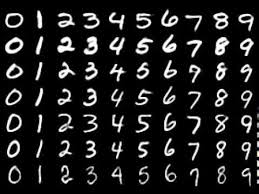
\includegraphics[height=.4\textheight]{mnist.jpeg}\hspace{2em}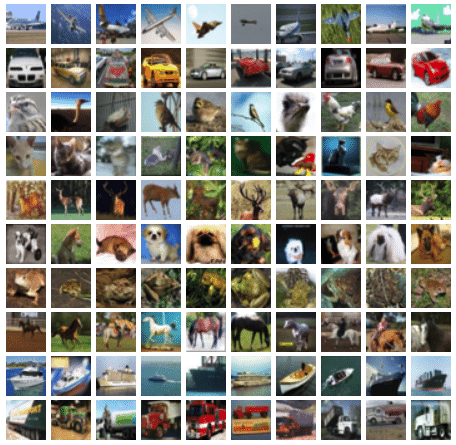
\includegraphics[height=.4\textheight]{cifar10.png}
\end{center}

\end{frame}

\begin{frame}[standout]
	\begin{center}
		\large preconditioning
	\end{center}
\end{frame}

\begin{frame}
	\frametitle{preconditioning}
	\textbf{Main idea:}
	Instead of minimizing $f(\bv{x})$, find another function $g(\bv{x})$ with the same minimum but which is better suited for first order optimization (e.g., has a smaller conditioner number).
	
	\vspace{2em}
	\textbf{Claim:} Let $h(\bv{x}): \R^d \rightarrow \R^d$ be an \emph{invertible function}. Let $g(\bv{x}) = f(h(\bv{x}))$. Then
	\begin{align*}
		\alert{\min_{\bv{x}} f(\bv{x})} &\alert{= \min_{\bv{x}} g(\bv{x})} & &\text{and} & \alert{\argmin_{\bv{x}} f(\bv{x})} &\alert{= h\left(\argmin_{\bv{x}} g(\bv{x})\right)}.
	\end{align*}
\end{frame}

\begin{frame}[t]
	\frametitle{preconditioning}
	\textbf{First Goal:} We need $g(\bv{x})$ to still be convex.
	
	\textbf{Claim:} Let $\bv{P}$ be an invertible $d\times d$ matrix and let $g(\bv{x}) = f(\bv{P}\bv{x})$. 
	\begin{center} 
		\alert{$g(\bv{x})$ is always convex.}
	\end{center}
\end{frame}

\begin{frame}[t]
	\frametitle{preconditioning}
	\textbf{Second Goal:} 
	
	$g(\bv{x})$ should have better condition number $\kappa$ than $f(\bv{x})$. 
	
	\textbf{Example:} 
	\begin{itemize}
		\item $f(\bv{x}) = \|\bv{A}\bv{x} - \bv{b}\|_2^2$. $\kappa_f =\frac{\lambda_1(\bv{A}^T\bv{A})}{\lambda_d(\bv{A}^T\bv{A})}$.
		\item $g(\bv{x}) = \|\bv{A}\bv{P}\bv{x} - \bv{b}\|_2^2$. $\kappa_g =\frac{\lambda_1(\bv{P}^T\bv{A}^T\bv{A}\bv{P})}{\lambda_d(\bv{P}^T\bv{A}^T\bv{A}\bv{P})}$.
	\end{itemize}
	
%	\textbf{Ideal preconditioner:} Choose $P$ so that  $\bv{P}^T\bv{A}^T\bv{A}\bv{P} = \bv{I}$. For example, could set $P = \sqrt{(\bv{A}^T\bv{A})^{-1}}$.
%	
%	\begin{center}
%		\alert{What's the problem with this choice?}
%	\end{center}
\end{frame}

\begin{frame}[t]
	\frametitle{diagonal preconditioner}
	\textbf{Third Goal:} $\bv{P}$ should be easy to compute. 
	
	\begin{center}
		\alert{Many, many problem specific preconditioners are used in practice. There design is usually a heuristic process.} 
	\end{center}
	
	\textbf{Example:} Diagonal preconditioner. 
	\begin{itemize}
		\item Let $\bv{D} = \diag(\bv{A}^T\bv{A})$
		\item Intuitively, we roughly have that $\bv{D} \approx \bv{A}^T\bv{A}$. 
		\item Let $\bv{P} = \sqrt{\bv{D}^{-1}}$
	\end{itemize}
	$\bv{P}$ is often called a \alert{\textbf{Jacobi preconditioner}}. Often works very well in practice!
\end{frame}

\begin{frame}
	\frametitle{diagonal preconditioner}
	\begin{center}
		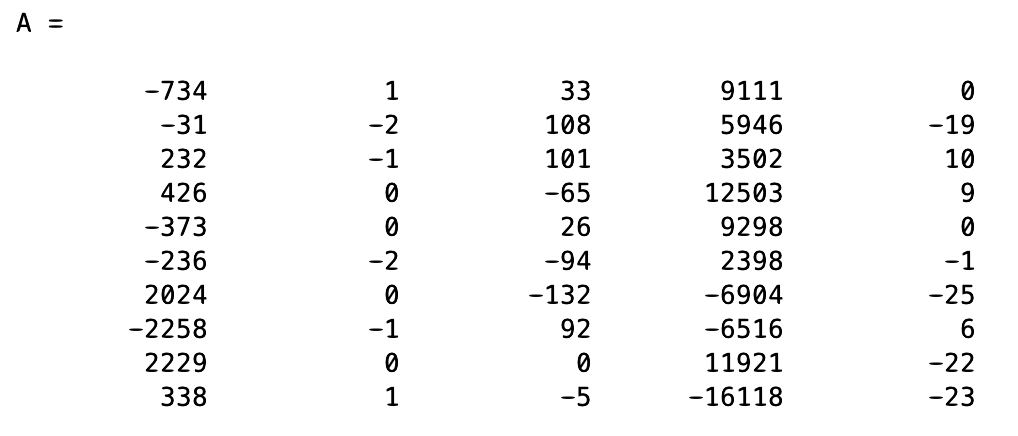
\includegraphics[width=.7\textwidth]{poorly_cond_a.png}
	\end{center}
	\vspace{2em}
	
	\begin{columns}[t]
		\begin{column}{0.3\textwidth}
			\vspace{-6.4em}
			
			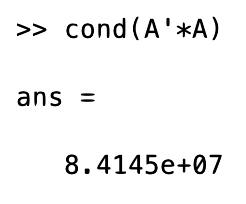
\includegraphics[width=.8\textwidth]{cond1.png}
		\end{column}
		\begin{column}{0.7\textwidth}
			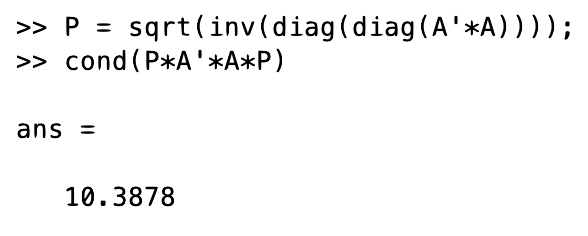
\includegraphics[width=.8\textwidth]{cond2.png}
		\end{column}
	\end{columns}
\end{frame}

%\begin{frame}
%	\frametitle{diagonal preconditioner}
%	\begin{center}
%		\alert{Can you think of an example $\bv{A}$ where Jacobi preconditioning doesn't decrease a large $\kappa$?}
%	\end{center}
%	\vspace{3em}
%		\begin{center}
%		\alert{Can Jacobi preconditioning \emph{increase} $\kappa$?}
%	\end{center}
%\end{frame}


\begin{frame}
	\frametitle{adaptive stepsizes}
	\textbf{Another view}: If $g(\bv{x}) = f(\bv{P}\bv{x})$ then $\nabla g(\bv{x}) = \bv{P}^T\nabla f(\bv{P}\bv{x})$.
	
	$\nabla g(\bv{x})  = \bv{P}\nabla f(\bv{P}\bv{x})$ when $\bv{P}$ is symmetric. 
	
	\vspace{1em}
	\textbf{Gradient descent on $g$:}
	\begin{itemize}
		\item For $t = 1,\ldots, T$,
		\begin{itemize}
			\item $\bv{x}^{(t+1)} = \bv{x}^{(t)} - \eta\bv{P}\left[\nabla f(\bv{P}\bv{x}^{(t)})\right]$
		\end{itemize}
	\end{itemize}
	
	\vspace{1em}
	\textbf{Gradient descent on $g$:}
	\begin{itemize}
		\item For $t = 1,\ldots, T$,
		\begin{itemize}
			\item $\bv{y}^{(t+1)} = \bv{y}^{(t)} - \eta\bv{P}^2\left[\nabla f(\bv{y}^{(t)})\right]$
		\end{itemize}
	\end{itemize}
	\begin{center}
		\alert{When $\bv{P}$ is diagonal, this is just gradient descent with a \emph{different step size for each parameter}!}
	\end{center}
\end{frame}

\begin{frame}
	\frametitle{adaptive stepsizes}
	\textbf{Algorithms based on this idea:}
	\begin{itemize}
		\item AdaGrad
		\item RMSprop
		\item Adam optimizer
	\end{itemize}
	\begin{center}
		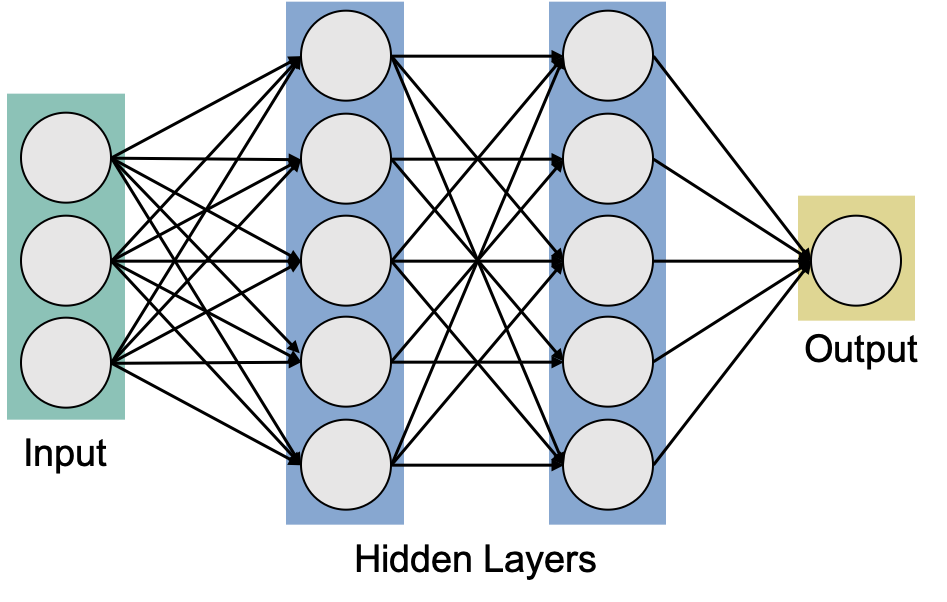
\includegraphics[width=.5\textwidth]{neuralNetwork.png}
		
		\alert{(Pretty much all of the most widely used optimization methods for training neural networks.)}
	\end{center}
\end{frame}

\begin{frame}[standout]
	\begin{center}
		\large coordinate descent
	\end{center}
\end{frame}

\begin{frame}
	\frametitle{stochastic methods}
	\textbf{Main idea:} Trade slower convergence (more iterations) for cheaper iterations. 
	\vspace{2em}
	
	\textbf{Stochastic Gradient Descent:}
	When $f(\bv{x}) = \sum_{i=1}^n f_i(\bv{x})$, approximate $\nabla f(\bv{x})$ with $\nabla f_i(\bv{x})$ for randomly chosen $i$. 
\end{frame}

\begin{frame}
	\frametitle{stochastic methods}
	\textbf{Main idea:} Trade slower convergence (more iterations) for cheaper iterations. 
	\vspace{2em}
	
	\textbf{Stochastic \alert{Coordinate Descent}:}
	Only compute a \emph{single random entry} of $\nabla f(\bv{x})$ on each iteration:
	\begin{align*}
		\nabla f(\bv{x}) &= 
		\begin{bmatrix}
			\frac{\partial f}{\partial x_1}(\bv{x}) \\ \frac{\partial f}{\partial x_2}(\bv{x}) \\ \vdots \\ \frac{\partial f}{\partial x_d}(\bv{x})  
		\end{bmatrix} & 	\nabla_i f(\bv{x}) &= 
		\begin{bmatrix}
			0\\ \frac{\partial f}{\partial x_i}(\bv{x}) \\ \vdots \\ 0
		\end{bmatrix} 
	\end{align*}
	
	\textbf{Update:} $\bv{x}^{(t+1)}\leftarrow \bv{x}^{(t)} + \eta \nabla_i f(\bv{x}^{(t)})$.
\end{frame}

%\begin{frame}[t]
%	\frametitle{coordinate descent}
%	When $\bv{x}$ has $d$ parameters, computing $\nabla_i f(\bv{x})$ often costs just a $1/d$ fraction of what it costs to compute $\nabla f(\bv{x})$ 
%	
%	\vspace{1em}
%	\textbf{Example:} $f(\bv{x}) = \|\bv{A}\bv{x} - \bv{b}\|_2^2$ for $\bv{A} \in \R^{n\times d}, \bv{x} \in \R^{d}, \bv{b} \in \R^n$. 
%	\begin{itemize}
%		\item $\nabla f(\bv{x}) = 2\bv{A}^T\bv{A}\bv{x} - 2\bv{A}^T\bv{b}$.
%		\item $\nabla_i f(\bv{x}) = 2\left[\bv{A}^T\bv{A}\bv{x}\right]_i - 2\left[\bv{A}^T\bv{b}\right]$.
%	\end{itemize}
%\end{frame}
%
%\begin{frame}[t]
%	\frametitle{stochastic coordinate descent}	
%	\textbf{Stochastic Coordinate Descent:}
%	\begin{itemize}
%		\item Choose number of steps $T$ and step size $\eta$.
%		\item For $i = 1,\ldots, T$:
%		\begin{itemize}
%			\item Pick random $j_i \in 1, \ldots, d$.
%			\item $\bv{x}^{(i+1)} = \bv{x}^{(i)} - \eta \nabla_{j_i} f(\bv{x}^{(i)})$
%		\end{itemize}
%		\item Return $\hat{\bv{x}} = \frac{1}{T}\sum_{i=1}^T \bv{x}^{(i)}$.
%	\end{itemize}
%\end{frame}
%
%\begin{frame}[t]
%	\frametitle{coordinate descent}
%	\begin{theorem}[Stochastic Coordinate Descent convergence]
%		Given a $G$-Lipschitz function $f$ with minimizer $\bv{x}^*$ and initial point $\bv{x}^{(1)} $ with $\|\bv{x}^{1)} - \bv{x}^*\|_2 \leq R$, SCD with step size $\eta = \frac{1}{Rd}$ satisfies the guarantee:
%		\begin{align*}
%			\E[f(\hat{\bv{x}}) - f({\bv{x}^*})] \leq \frac{2GR}{\sqrt{T/d}}
%		\end{align*}
%	\end{theorem}
%\end{frame}
%
%\begin{frame}[t]
%	\frametitle{importance sampling}
%	Often it doesn't make sense to sample $i$ uniformly at random:
%	\begin{align*}
%		\bv{A} &= \begin{bmatrix} 
%			0 & 0 & 1 & 0 & 0 & 0 \\
%			0 & 0 & 2 & 0 & 0 & 0 \\
%			0 & 0 & -1 & 0 & 0 & 0 \\
%			0 & 0 & -.5 & 0 & 0 & 0 \\
%			0 & 0 & 3 & 0 & 0 & 0 \\
%			0 & 0 & -2 & 0 & 0 & 0 
%		\end{bmatrix} & 
%		\bv{b} &=\begin{bmatrix} 
%			10  \\
%			42 \\
%			-11  \\
%			-51 \\
%			34\\
%			-22 
%		\end{bmatrix} 
%	\end{align*}
%	Select indices $i$ proportional to $\|\bv{a}_i\|_2^2$:
%	\begin{align*}
%		\Pr[\text{select index $i$ to update}] = \frac{\|\bv{a}_i\|_2^2}{\sum_{j=1}^d \|\bv{a}_j\|_2^2} = \frac{\|\bv{a}_i\|_2^2}{\|\bv{A}\|_2^2} 
%	\end{align*}
%\end{frame}



%\begin{frame}[t]
%	\frametitle{in-class exercise}
%	\begin{theorem}[GD for $\beta$-smooth, $\alpha$-strongly convex.]
%		Let $f$ be a $\beta$-smooth and $\alpha$-strongly convex function. If we run GD for $T$ steps (with step size $\eta = \frac{1}{\beta}$) we have:
%		\begin{align*}
%			\|\bv{x}^{(t)} - \bv{x}^*\|_2^2 \leq e^{-(t-1)\frac{\alpha}{\beta}} \|\bv{x}^{(0)} - \bv{x}^*\|_2^2
%		\end{align*} 
%	\end{theorem}
%	
%	\begin{center}
%		\alert{\textbf{Prove for $f(\bv{x}) = \|\bv{D}\bv{x} - \bv{b}\|_2^2$.}}
%	\end{center}	
%	
%\end{frame} 
%
%\begin{frame}[t]
%	\frametitle{in-class exercise}
%\end{frame}
%
%\begin{frame}[t]
%	\frametitle{in-class exercise}
%\end{frame}

\end{document} 








